%%
%% Copyright 2007-2020 Elsevier Ltd
%%
%% This file is part of the 'Elsarticle Bundle'.
%% ---------------------------------------------
%%
%% It may be distributed under the conditions of the LaTeX Project Public
%% License, either version 1.2 of this license or (at your option) any
%% later version.  The latest version of this license is in
%%    http://www.latex-project.org/lppl.txt
%% and version 1.2 or later is part of all distributions of LaTeX
%% version 1999/12/01 or later.
%%
%% The list of all files belonging to the 'Elsarticle Bundle' is
%% given in the file `manifest.txt'.
%%
%% Template article for Elsevier's document class `elsarticle'
%% with harvard style bibliographic references

%\documentclass[preprint,12pt,authoryear]{elsarticle}

%% Use the option review to obtain double line spacing
%% \documentclass[authoryear,preprint,review,12pt]{elsarticle}

%% Use the options 1p,twocolumn; 3p; 3p,twocolumn; 5p; or 5p,twocolumn
%% for a journal layout:
%% \documentclass[final,1p,times,authoryear]{elsarticle}
%% \documentclass[final,1p,times,twocolumn,authoryear]{elsarticle}
%% \documentclass[final,3p,times,authoryear]{elsarticle}
%% \documentclass[final,3p,times,twocolumn,authoryear]{elsarticle}
%% \documentclass[final,5p,times,authoryear]{elsarticle}
 \documentclass[final,5p,times,twocolumn,authoryear]{elsarticle}


%% For including figures, graphicx.sty has been loaded in
%% elsarticle.cls. If you prefer to use the old commands
%% please give \usepackage{epsfig}

%% The amssymb package provides various useful mathematical symbols
\usepackage{xcolor}        % <- só depois podes importar pacotes
\usepackage{amssymb}
\usepackage{amsmath}
\usepackage{xcolor}
\usepackage{float}


%% The amsthm package provides extended theorem environments
%% \usepackage{amsthm}

%% The lineno packages adds line numbers. Start line numbering with
%% \begin{linenumbers}, end it with \end{linenumbers}. Or switch it on
%% for the whole article with \linenumbers.
%% \usepackage{lineno}

\usepackage{titlesec}
\titleformat{\section}{\bfseries\large}{\thesection}{1em}{}
\titleformat{\subsection}{\bfseries\normalsize}{\thesubsection}{1em}{}
\titleformat{\subsubsection}{\bfseries\normalsize}{\thesubsubsection}{1em}{}


\begin{document}


\begin{frontmatter}

\title{WE NEED A TITLE HEERE ???}

\author[first]{Leonor Ramos}
\author[second]{Tiago Patrício}
\author[third]{João Almeida}
\author[fourth]{David Mendes}
\affiliation{organization={ISCTE – Instituto Universitário de Lisboa}, country={Portugal}} % Title page setup



\begin{abstract}
\chapter*{Resumo}

Write here your abstract in Portuguese
\textbf{keywords} \begin{keyword}key1 \sep key2 \sep key3 \end{keyword}
\par
\chapter*{Abstract}
Write here your abstract in English
\par
\textbf{keywords} \begin{keyword}key1 \sep key2 \sep key3 \end{keyword}
\end{abstract}


\end{frontmatter}

%\tableofcontents

%% \linenumbers

%% main text


\section{Introduction}
\label{introduction}

This project was developed in two distinct parts, with the common goal of creating an autonomous controller for the Thymio robot, capable of exploring environments while avoiding collisions with obstacles and falls from cliffs.

In the first part, more traditional control methods were explored, based on evolutionary algorithms and artificial neural networks (ANNs). Initially, an approach based on Braitenberg machines was implemented, using simple connections between sensors and actuators to generate reactive behaviors. Subsequently, simple neural networks were developed, using only the ground sensors. The next step involved the development of more advanced neural networks that combined ground sensors with front-facing proximity sensors, allowing for obstacle avoidance. These approaches enabled the study of the robot’s response to different sensory configurations and simple control strategies.

In the second part of the project, we explored the use of Deep Reinforcement Learning algorithms, specifically the Proximal Policy Optimization (PPO) algorithm, to train a more sophisticated controller. The goal was to enable the robot, starting from the central area of the environment and with any initial orientation, to efficiently explore the space while avoiding collisions and cliff falls. To achieve this, a neural network was used that, based on sensor observations — five front-facing proximity sensors and two downward-facing ground sensors — learned to determine the speed of each robot wheel in order to maximize safe and effective exploration performance.

This integrated approach allowed for a comparison between classical and modern robotic control techniques, evaluating their robustness, generalization ability, and effectiveness in autonomous navigation in complex environments.

\section{Methodology}

This section focuses on the approaches implemented to develop effective autonomous behavior in the Thymio robot. Both classical solutions based on evolutionary algorithms and artificial neural networks, as well as modern techniques involving Deep Reinforcement Learning, were explored.



\subsection{\textbf{Part A: Classical approaches based on evolutionary algorithms and artificial neural networks}}

In the first phase of the project, classical behavioral control approaches were implemented and tested using evolutionary algorithms and artificial neural networks (ANNs).

The experiments in Part A were conducted in a fixed, predefined simulation environment featuring a black line path over a white floor and optionally static obstacles. This environment was specifically designed to test basic reactive behaviors and assess line-following and obstacle avoidance capabilities under controlled conditions.

\begin{figure}[H]
    \centering
    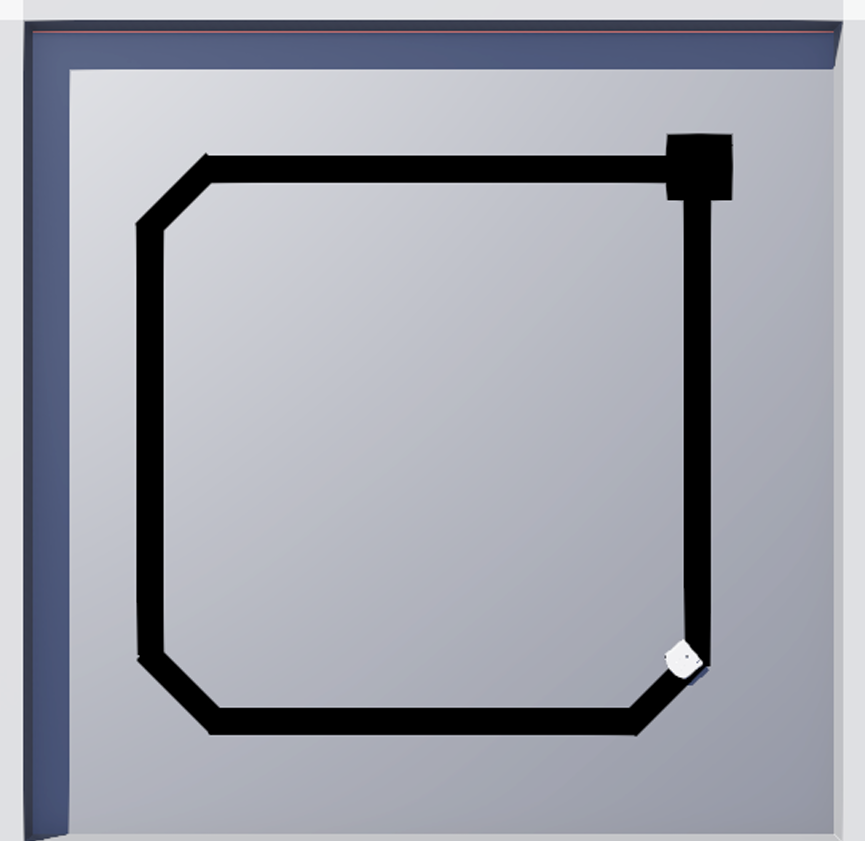
\includegraphics[width=0.25\textwidth]{figures/env1.png}
    \caption{Simulation environment used for Part A (Evolutionary approaches).}
    \label{fig:env1}
\end{figure}

\subsubsection{Phase 1: Evolutionary Braitenberg Machine}

The objective of this phase was to develop a simple reactive controller based on the concept of a Braitenberg Machine, with its parameters optimized using an Evolutionary Algorithm (EA).

The controller architecture consists of two ground sensors as input (left and right) and two outputs corresponding to the left and right motor speeds. The motor speeds are calculated through linear equations that combine the sensor readings with weighted parameters, as follows:

\begin{equation}
    \text{Left\_Motor} = (P_{1L} \cdot S_L) + (P_{2L} \cdot S_R) + P_{3L}
\end{equation}    
\begin{equation}
    \text{Right\_Motor} = (P_{1R} \cdot S_L) + (P_{2R} \cdot S_R) + P_{3R}
\end{equation} 

, where \(S_L\) and \(S_R\) represent the readings from the left and right ground sensors, respectively. In total, there are six parameters to be optimized: three for the left motor (\(P_{1L}, P_{2L}, P_{3L}\)) and three for the right motor (\(P_{1R}, P_{2R}, P_{3R}\)).

These parameters were evolved with the goal of maximizing the robot's performance in the exploration task, keeping it in motion and avoiding cliff falls, relying solely on the information provided by the ground sensors.

Initially, a population of controllers with randomly generated weights was created. For each generation, the evolutionary process involved the following steps:

\begin{itemize}
    \item Each individual controller was evaluated by simulating its behavior and measuring its performance, expressed as fitness.
    \item The best-performing individuals were selected to act as parents for the next generation.
    \item New individuals were generated from these parents using crossover and mutation operations.
    \item The average fitness of the population for the generation was recorded.
\end{itemize}

The fitness function was designed to reward behaviors that keep the robot over the black line. At each simulation step, the readings from the two ground sensors were analyzed. The function increased the fitness score whenever the robot was correctly positioned on the line — with greater rewards if both sensors detected the black line simultaneously. The total fitness of an individual is the accumulated score over the evaluation time, normalized as:

\begin{equation}
    fitness= \frac{\text{\textit{Time on Line}}}{\text{\textit{Evaluation Time}}}
\end{equation}

This encourages solutions that can consistently follow the line throughout the simulation.

The parameters used in the genetic algorithm were:

\begin{itemize}
    \item \textbf{Population size}: 10 individuals
    \item \textbf{Generations}: 300
    \item \textbf{Elitism}: The top 3 individuals (based on fitness) are preserved in each generation
    \item \textbf{Crossover}: One-point crossover between parent weight vectors
    \item \textbf{Mutation}: Each gene has a 20\% chance of being mutated with Gaussian noise ( $\sigma = 0.05$)
    \item \textbf{Genome representation}: 6 floating-point weights, corresponding to the motor control equations
\end{itemize}

The evolutionary algorithm optimized the parameters over generations, producing a Braitenberg-style controller capable of navigating by following the black line using only ground sensor inputs.

% Cole este bloco de código no seu ficheiro .tex principal, no local desejado.
% Para os comandos matemáticos como \text e \underbrace, certifique-se que tem o
% pacote amsmath incluído no seu preâmbulo: \usepackage{amsmath}

% Cole este bloco de código no seu ficheiro .tex principal.
% Certifique-se que tem o pacote amsmath incluído: \usepackage{amsmath}

\subsubsection{Phase 2: Simple ANN (Ground Sensors Only)}

The objective of this phase was to evolve a minimalistic artificial neural network (ANN) for a complex task involving both initial exploration and subsequent line-following, constrained to using only the robot’s two ground sensors.

The network architecture was strictly defined as follows:
\begin{itemize}
    \item \textbf{Inputs:} Two normalized values from the ground sensors.
    \item \textbf{Hidden Layer:} Four neurons with hyperbolic tangent (\textit{tanh}) activation.
    \item \textbf{Outputs:} Two neurons, also with \textit{tanh} activation, controlling the left and right motor speeds.
\end{itemize}

The network's 22 parameters, encompassing all weights and biases, were subject to evolutionary optimization:
\[
\underbrace{(2 \times 4)}_{\text{input-to-hidden weights}} + \underbrace{4}_{\text{hidden biases}} + \underbrace{(4 \times 2)}_{\text{hidden-to-output weights}} + \underbrace{2}_{\text{output biases}}
\]

Raw sensor values were normalized to the range \([-1, 1]\). The network outputs were then scaled to motor speeds to ensure continuous forward motion using the formula:
\begin{equation}
    \text{speed} = \text{BASE\_SPEED} + \text{output} \times (\text{MAX\_SPEED} - \text{BASE\_SPEED})
    \label{eq:speed_scaling}
\end{equation}
where $\text{BASE\_SPEED} = 3.0$ and $\text{MAX\_SPEED} = 6.28$.

A primary challenge in this phase is the robot's ``perceptual blindness'' when off the line, as the sensors provide no directional information for search. To guide the evolution, a \textbf{shaped fitness function} was employed, consisting of two components:
\begin{itemize}
    \item \textbf{Execution Fitness ($F_{\text{exec}}$):} This component rewards the \textbf{distance traveled} while on the line, weighted by a multiplier of 1.0 for being centered (both sensors on the line) and 0.5 for partial contact (one sensor on the line).
    
    \item \textbf{Exploration Fitness ($F_{\text{expl}}$):} A fixed bonus with a maximum value of 10.0 is awarded for \textbf{finding the line quickly}. The bonus is scaled by the proportion of evaluation time remaining after the first contact is made.
\end{itemize}

The total fitness for an individual is the sum of these two components:
\begin{equation}
    \text{Fitness}_{\text{total}} = F_{\text{exec}} + F_{\text{expl}}
    \label{eq:total_fitness}
\end{equation}

The network parameters were evolved using a Genetic Algorithm (GA) featuring an \textbf{adaptive mutation strategy}. This strategy was designed to balance broad exploration in early generations with fine-tuning in later stages. The GA was configured as follows:
\begin{itemize}
    \item \textbf{Population Size:} 30 individuals
    \item \textbf{Generations:} 300
    \item \textbf{Selection:} The top 4 individuals are selected as parents for reproduction.
    \item \textbf{Elitism:} A single-best elitism strategy was used, where the top-performing individual from each generation is guaranteed to pass, unaltered, to the next.
    \item \textbf{Crossover:} Single-point crossover between two randomly selected parents from the elite group.
    \item \textbf{Adaptive Mutation:} Both the mutation rate and size decrease linearly over the first 75\% of generations. The mutation rate anneals from 0.25 to 0.05, and the mutation size (standard deviation of Gaussian noise) anneals from 0.5 to 0.1.
\end{itemize}

To ensure the development of robust and generalizable behaviors, the robot’s starting position and orientation were fully randomized within the arena before each 200-second evaluation period. This methodology combines a simple reactive controller with a sophisticated evolutionary optimization process to address the challenges of learning with limited sensory information.



\subsubsection{Phase 3: Advanced Artificial Neural Network (Ground Sensors + Obstacles)}

The network architecture was expanded to include five inputs: two ground sensors and three front proximity sensors. The hidden layer consisted of 4 neurons with hyperbolic tangent (\textit{tanh}) activation, and the output layer had 2 neurons corresponding to the left and right motor speeds. The increased number of inputs raised the total parameters subject to optimization to 34, calculated as:

\[
\underbrace{5 \times 4}_{\text{input-to-hidden weights}} + \underbrace{4 \times 2}_{\text{hidden-to-output weights}} + \underbrace{4 + 2}_{\text{biases for hidden and output layers}}
\]

To harmonize sensor data, raw proximity sensor readings were linearly normalized to the \([0,1]\) interval, consistent with the normalization applied to ground sensors. This enabled the network to integrate terrain and obstacle information effectively.

Given the increased task complexity, the evolutionary algorithm parameters were adjusted: the population size was increased, and the number of generations extended to facilitate convergence. The fitness function was enhanced to evaluate both line-following performance and obstacle avoidance, penalizing collisions to promote safe navigation.

The evaluation environment incorporated fixed obstacles along the track, simulating real-world challenges. Performance metrics accounted for the robot’s ability to maintain line tracking without collisions and encouraged smooth navigation trajectories, guiding the evolution of more sophisticated control behaviors.

To guide the evolutionary process, a multi-objective fitness function was implemented, balancing three key performance indicators: line-following accuracy, obstacle avoidance, and area coverage. The function is defined as:

\begin{equation}
    fitness= w_{line} \dot S_{line} + w_{obstacle} \dot S_{obstacle} + w_{area} + S_{area} - P
\end{equation}

, where:

\begin{itemize}
    \item $S_{line}$ is the proportion of time the robot remained on the line,

    \item $S_{obstacle}$ is the proportion of time without collisions

    \item $S_{area}$ is the ratio of distance covered to the maximum possible distance,

    \item  $ w_{line}$, $w_{obstacle}$, $w_{area}$ are the respective weights for each objective,

    \item $P$ is the total penalty applied for poor performance in any of the objectives.
\end{itemize}

Penalties were introduced to discourage undesirable behaviors:

\begin{itemize}
    \item A collision penalty was applied if the number of collisions exceeded a predefined threshold.

    \item An off-line penalty was triggered if the robot spent less than 5\% of the time on the line.

    \item An area penalty was applied when the robot covered less than 20\% of the expected distance.
\end{itemize}

All scores were clamped to the 
[0,1] interval to ensure stability and comparability across different runs. The final fitness value was also clamped to a minimum of zero to prevent negative values from disrupting the evolutionary process.

%\paragraph{Implementation and Evaluation}

%The fitness function was implemented in Python and integrated into the evolutionary loop. During each generation, individuals were evaluated in a simulated environment with fixed obstacles and a predefined track. The simulation recorded metrics such as time on line, number of collisions, and distance traveled. These metrics were then passed to the fitness function to compute the score.

%This approach allowed the evolutionary algorithm to favor individuals that demonstrated balanced behavior—accurately following the line, avoiding obstacles, and exploring the environment efficiently. The printed logs during evaluation provided transparency and facilitated debugging and tuning of the fitness function.






\subsection{Part B: PPO Implementation}

In the second part of the project, a Deep Reinforcement Learning (DRL) approach was adopted using the Proximal Policy Optimization (PPO) algorithm. The objective was to train a more robust and generalizable policy capable of navigating a dynamic environment, avoiding both obstacles and cliff edges.

The environment, shown in Figure~\ref{fig:env_ppo}, was designed with a static H-shaped track layout but featured dynamically positioned obstacles. This setup, known as \textit{domain randomization}, forces the agent to learn general strategies for obstacle avoidance rather than memorizing a single static path.

\begin{figure}[H]
    \centering
    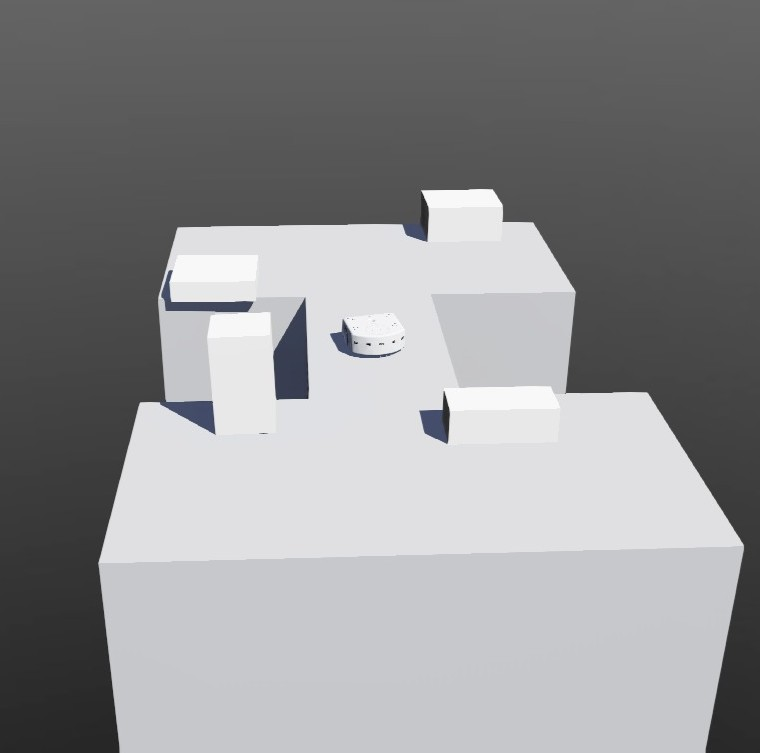
\includegraphics[width=0.45\textwidth]{figures/env2.png}
    \caption{Simulation environment used for training the PPO agent, featuring an H-shaped track and randomized obstacle placement.}
    \label{fig:env_ppo}
\end{figure}

\subsubsection{Reinforcement Learning Framework}

The problem was framed within the standard reinforcement learning paradigm, where an agent interacts with an environment to maximize a cumulative reward signal.

\begin{itemize}
    \item \textbf{State and Action Spaces}
        The agent's perception and interaction with the world were defined as follows:
        \begin{itemize}
            \item \textbf{Observation Space:} A 7-dimensional continuous vector containing normalized sensor readings. This included five frontal proximity sensors to detect obstacles and two ground sensors to detect the track edges. Each sensor value was normalized to a range of \([0, 1]\).
            \item \textbf{Action Space:} A 2-dimensional continuous space, where each value in the range \([-1, 1]\) corresponds to the normalized velocity for the left and right motors, respectively.
        \end{itemize}
    \item \textbf{Policy Network Architecture}
        The agent's "brain" is a policy network implemented as a Multi-Layer Perceptron (MLP). The PPO algorithm, sourced from the Stable-Baselines3 library, was used to train this network. The architecture was configured as follows:
        \begin{itemize}
            \item \textbf{Input Layer:} 7 neurons, corresponding to the observation space.
            \item \textbf{Hidden Layers:} Two hidden layers with 64 and 32 neurons, respectively, using the ReLU and Tanh activation functions.
            \item \textbf{Output Layer:} 2 neurons, producing the continuous values for the action space.
        \end{itemize}
    \item \textbf{Reward Engineering}
        The success of the DRL agent is critically dependent on the design of the reward function. A carefully shaped reward signal was engineered to encourage the desired emergent behaviors:
        \begin{itemize}
            \item \textbf{Catastrophic Failure Penalty:} A large negative reward of \(-100\) is given if the agent falls off the track. This is detected either by a low ground sensor reading or a significant drop in the robot's z-axis coordinate. This event immediately terminates the episode.
            \item \textbf{Movement and Exploration Incentive:} A positive reward proportional to the distance traveled in each step ($+20 \times \text{distance}$) encourages the agent to actively move and explore the environment, penalizing immobility.
            \item \textbf{Proximity-Based Collision Avoidance:} A progressive negative penalty is applied as the robot gets closer to obstacles. The penalty is proportional to the sum of proximity sensor readings that exceed a threshold of 0.5, discouraging the agent from lingering near walls.
            \item \textbf{Survival Bonus:} A small, constant positive reward of \(+0.5\) is given at each step the agent survives without failure, incentivizing longevity.
            \item \textbf{Episode Completion Bonus:} A large positive reward of \(+200\) is awarded if the agent successfully survives for the entire maximum duration of an episode, strongly reinforcing robust, long-term survival strategies.
        \end{itemize}
    \item \textbf{Training Process and Generalization}
        The training process was configured to promote robust and generalizable policies.
        \begin{itemize}
            \item \textbf{Algorithm:} Proximal Policy Optimization (PPO).
            \item \textbf{Hyperparameters:} A learning rate of \(3 \times 10^{-4}\) and an entropy coefficient (\texttt{ent\_coef}) of \(0.01\) were used to balance policy optimization with exploration.
            \item \textbf{Domain Randomization:} At the start of each episode, the positions, orientations, and sizes of the five obstacles were randomized. This prevents the agent from overfitting to a single environment configuration and forces it to learn a more general obstacle avoidance policy.
            \item \textbf{Normalization:} The \texttt{VecNormalize} wrapper from Stable-Baselines3 was used to normalize both observations and rewards during training, a standard technique for stabilizing the learning process in DRL.
            \item \textbf{Training Duration:} The agent was trained for a total of 100,000 timesteps, with model checkpoints saved periodically.
        \end{itemize}
\end{itemize}

\subsubsection{Phase 2: Recurrent Policy Optimization}

Building upon the foundation of the first DRL phase, the second phase addressed a key limitation of the standard feedforward policy: its lack of temporal memory. While the `MlpPolicy` reacts only to the immediate sensory input, many real-world navigation challenges benefit from understanding the recent history of observations and actions. To this end, a recurrent policy was implemented.

The core change in this phase was the adoption of the \textbf{Recurrent Proximal Policy Optimization (RecurrentPPO)} algorithm, a variant of PPO designed to train policies with memory. This was paired with a corresponding recurrent network architecture.

\begin{itemize}
    \item \textbf{Recurrent Policy Network (\textit{MlpLstmPolicy})}
        The key innovation in this phase is the introduction of a \textbf{Long Short-Term Memory (LSTM)} layer into the policy network. The \textit{MlpLstmPolicy} architecture maintains a hidden state that is updated at each timestep, allowing it to integrate information over time. This enables the agent to learn from sequences of observations, rather than just instantaneous snapshots.
        
    \item \textbf{Environment and Reward Structure}
        The underlying simulation environment, including the state/action spaces and the carefully engineered reward function, remained identical to the one used in the first PPO phase. This controlled setup ensures that any observed differences in performance can be directly attributed to the change in the policy's architecture—from a reactive \textit{MlpPolicy} to a memory-aware \textit{MlpLstmPolicy}.

    \item \textbf{Training Configuration}
        The training process was adapted to accommodate the recurrent nature of the model, while keeping other key parameters consistent for a fair comparison:
        \begin{itemize}
            \item \textbf{Algorithm:} Recurrent Proximal Policy Optimization (RecurrentPPO), from the \texttt{sb3-contrib} library.
            \item \textbf{Policy Architecture:} `MlpLstmPolicy`, which incorporates an LSTM layer alongside the MLP feature extractor.
            \item \textbf{Hyperparameters:} The learning rate (\(3 \times 10^{-4}\)) and entropy coefficient (0.01) were kept consistent with the previous phase.
            \item \textbf{Training Duration:} The total number of timesteps was increased to 300,000 to provide sufficient time for the more complex recurrent policy to converge.
        \end{itemize}

\end{itemize}


This phase aims to demonstrate whether the introduction of recurrent memory can lead to a more stable, intelligent, and robust navigation policy compared to the purely reactive agent from the preceding experiment.





\section{Results}

Here we analyze and discuss several different results for different parameters of the different algorithms, any relevant graphs not included here have been added to the Appendix (see \ref{sec:appendix})

\subsection{Evolutionary Braitenberg Machine}

The application of the Evolutionary Braitenberg Machine was very successful in creating an agent capable of following the line. 

There is a clear overall increase in fitness across generations, indicating that the evolutionary algorithm progressively improves the controllers' ability to complete the task (staying on the line) and gaining better fitness.

As per the requirements, the robots were trained with two sets of parameters for comparison:

\begin{itemize}
    \item Parameters1, as in Fig. \ref{fig:evolv-params1}
    \begin{verbatim}
    # ...
    MUTATION_RATE = 0.2
    MUTATION_SIZE = 0.05
    # ...
    \end{verbatim}
    
    \item Parameters2, as in Fig. \ref{fig:evolv-params2}
    \begin{verbatim}
    # ...
    MUTATION_RATE = 0.3
    MUTATION_SIZE = 0.1
    # ...
    \end{verbatim}
\end{itemize}

Where MUTATION\_RATE controls if a gene (a single weight) mutates, while MUTATION\_SIZE controls how much a gene mutates.

% \begin{figure}[htbp] % Or [H] if you've added the float package and need absolute placement
%     \centering
%     \includegraphics[width=0.5\linewidth]{images/innerOutterGraph.png}
%     \caption{Base optimizer and Mesa optimizer}
%     \label{fig:architectureImage} % Label should typically be after caption
%     \source{\cite{RobertMilesAISafety2021MesaOptimizers}} % Or the actual source
% \end{figure}

\begin{figure}[H]
    \centering
    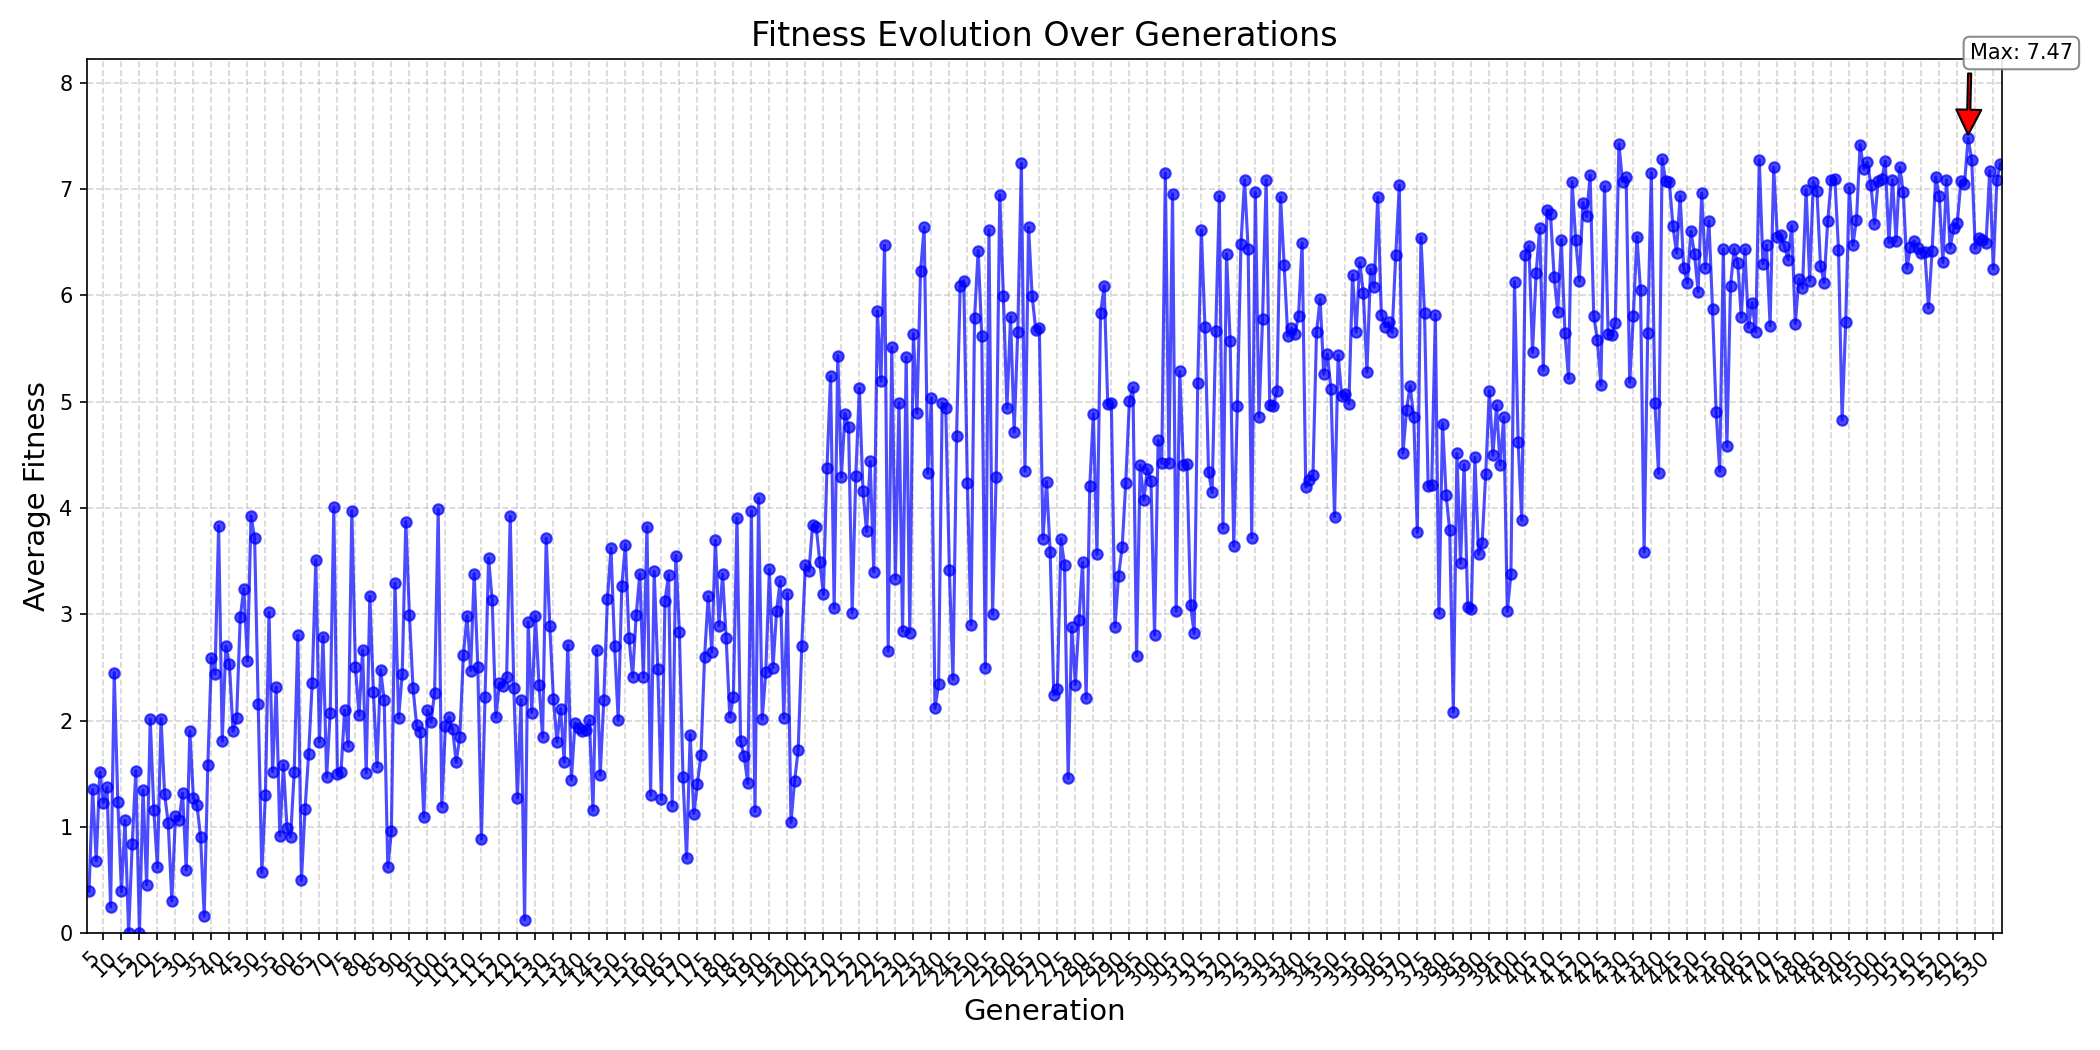
\includegraphics[width=1\linewidth]{figures/evolutivo_params_1.png}
    \caption{Evolutionary Algorithm: Average Fitness Across Generations – Parameters 1}
    \label{fig:evolv-params1}
\end{figure}

\begin{figure}[H]
    \centering
    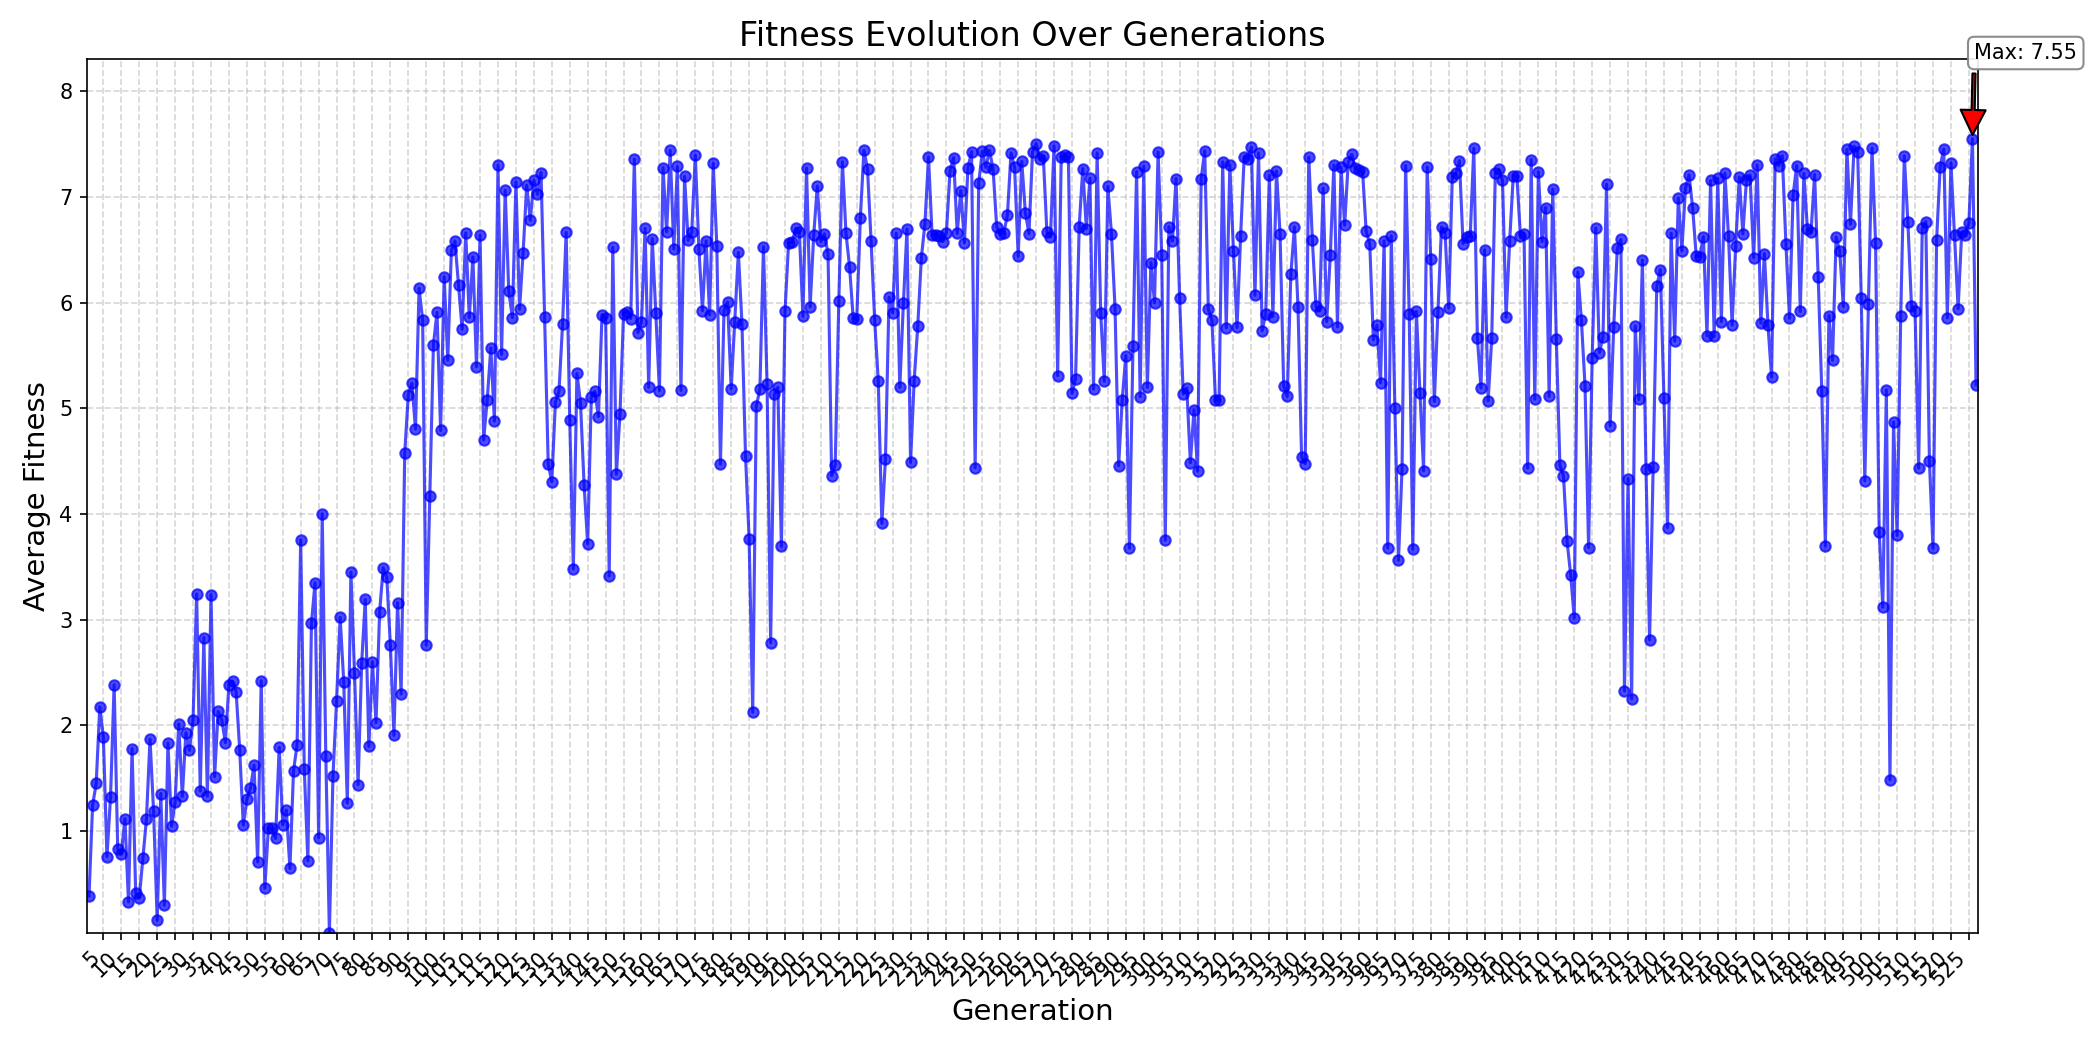
\includegraphics[width=1\linewidth]{figures/evolutivo_params2.png}
    \caption{Evolutionary Algorithm: Average Fitness Across Generations – Parameters 2}
    \label{fig:evolv-params2}
\end{figure}

As we can see, having a higher mutation rate and mutation size made it possible for our agent to learn much faster (it stagnated almost 300 generations before Fig. \ref{fig:evolv-params1}!), this shows just how much tuning small parameters can change the behavior and performance of the robot during and after training.

Despite this, the evolutionary method still exhibits a lot of variation in the average fitness accross generations, this can be attributed to factors like:

\begin{itemize}
    \item Random initial starting position and direction of the robot, witch influences it's fitness.
    
    \item Mutation and crossover operators introduce diversity, which can lead to both improvements and regressions in fitness.
    
    \item Small variations lead to big differences in the time spent in the line and thus the fitness of the robot.
\end{itemize}

% \begin{figure}[H]
%     \centering
%     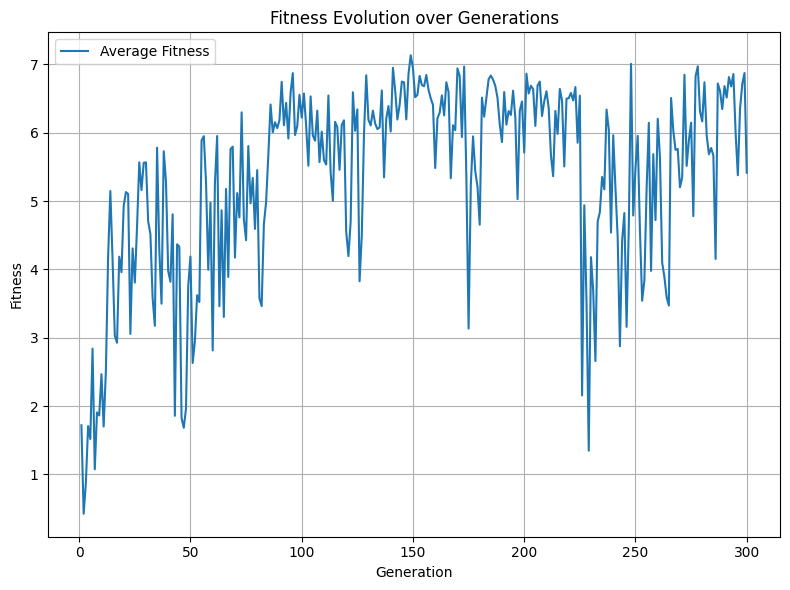
\includegraphics[width=0.4\textwidth]{figures/fitnessmb.png}
%     \caption{Fitness evolution over generations: evolutionary Braitenberg machine}
%     \label{fig:env_ppo}
% \end{figure}

% There is a clear overall increase in fitness across generations, indicating that the evolutionary algorithm progressively improves the controllers' ability to complete the task (staying on the line). However, the graph exhibits significant fluctuations, with many peaks and sudden drops, reflecting some instability in performance evaluation. This instability can be attributed to several factors:

% \begin{itemize}
%     \item \textbf{Random initial conditions:} The robot’s randomized starting position and orientation in each evaluation directly influence individual performance, causing natural variation in fitness scores.
    
%     \item \textbf{Stochastic nature of the evolutionary process:} Mutation and crossover operators introduce genetic diversity, which can lead to both improvements and regressions in fitness from one generation to another, producing peaks and valleys.
    
%     \item \textbf{Fitness based on time spent on target:} Small differences in robot behavior can result in large variations in the time spent on the line, impacting the fitness calculation accordingly.
% \end{itemize}

% Despite this variability, the positive trend confirms the method’s ability to evolve better controllers over time, while emphasizing the necessity of multiple runs to ensure robustness and reliable conclusions.

% Cole esta secção no seu ficheiro .tex
% Lembre-se de ter \usepackage{graphicx} e \usepackage{amsmath} no seu preâmbulo.

\subsection{Simple ANN Results}

The evolution of the simple ANN controller was monitored over 300 generations. The results, depicted in Figure~\ref{fig:ANN_full} and Figure~\ref{fig:ANN_zoom}, reveal a distinct two-phase evolutionary process: a period of rapid initial learning followed by a phase of high volatility and performance stagnation.

\begin{figure}[H]
    \centering
    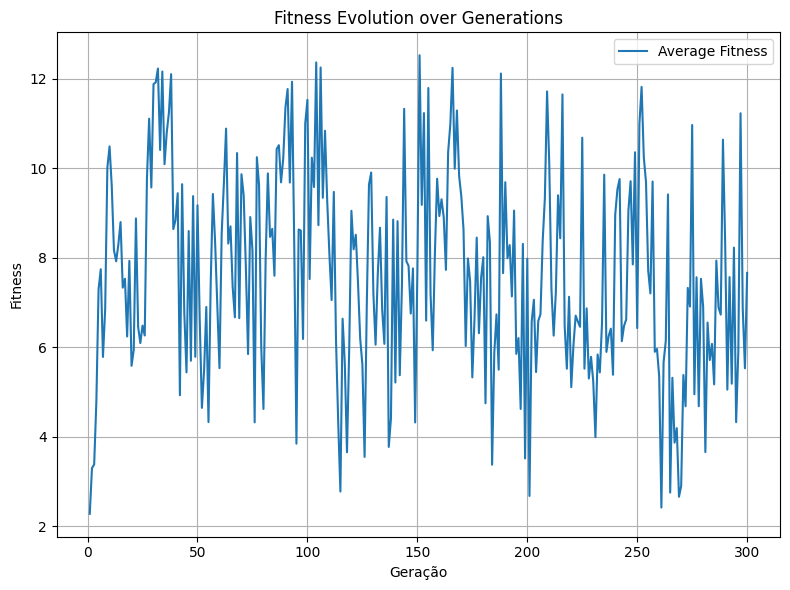
\includegraphics[width=0.4\textwidth]{figures/ANN_Simple_MutationVariable.png}
    \caption{Average fitness evolution over 300 generations. The graph shows high volatility and a lack of consistent long-term improvement after an initial learning phase.}
    \label{fig:ANN_full}
\end{figure}

\begin{figure}[H]
    \centering
    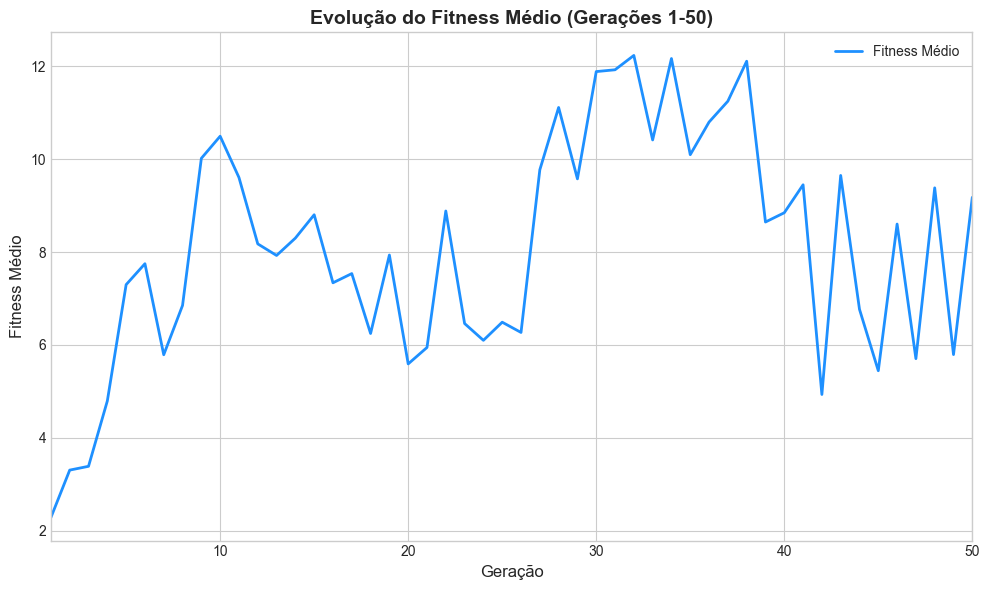
\includegraphics[width=0.4\textwidth]{figures/ANN_MUtationVariable_ChangedWindow.png}
    \caption{A focused view of the first 50 generations, highlighting the rapid and consistent increase in average fitness as the population first learns to solve the exploration task.}
    \label{fig:ANN_zoom}
\end{figure}
\begin{itemize}
    \item \textbf{Rapid Initial Learning (Generations 1-50)}
    As shown in Figure~\ref{fig:ANN_zoom}, the initial phase of evolution is characterized by a steep and consistent rise in average fitness, increasing from approximately 2.0 to peaks exceeding 12.0. This rapid improvement demonstrates the effectiveness of the shaped fitness function. The large exploration bonus ($F_{\text{expl}}$), combined with the high initial parameters of the adaptive mutation strategy, strongly incentivized the discovery of any behavior that resulted in finding the line. During this stage, the primary evolutionary pressure was to solve the exploration problem, which the genetic algorithm achieved successfully.

    \item  \textbf{Performance Volatility and Stagnation (Generations 50-300)}
Following the initial learning phase, the global view in Figure~\ref{fig:ANN_full} shows that the average fitness fails to converge to a stable, high value. Instead, it exhibits extreme volatility, oscillating between high peaks and deep troughs. This behavior reveals a fundamental conflict between the two objectives of the task: exploration and execution.

The high-scoring individuals evolved into "specialists" proficient at line-following ($F_{\text{exec}}$). However, these specialized behaviors were often ineffective for exploration. Due to the randomized starting positions, these specialists would frequently fail to find the line at all, resulting in a fitness score of zero and causing the population's average fitness to plummet in subsequent generations.

Ultimately, this volatility is a direct consequence of the ANN's architectural simplicity. With only two inputs and no internal memory, the network is incapable of context-aware behavior; it cannot differentiate between being "lost far from the line" and "just falling off the line" to switch between searching and following strategies. The resulting reactive behaviors are inherently brittle, leading to the observed performance instability. The results do not signify a failure of the evolutionary process, but rather successfully characterize the performance limitations of a simple reactive controller on a complex task.
\end{itemize}
\subsection{Advanced ANN (Ground Sensors + Obstacles)}
For the advanced ANN, 3 proximity sensors were used we choose sensors 0, 2, and 4 and we verified for collisions with 3 states if below 3000 for no collisions, between 4000 > value > 3000 for near a collision and if > 4000 we assumed there was a collision, to monitor for collisions we used all proximity sensors with value > 4300, for the line we used a similar method to the simple ANN where is multiplies a reward with the distance walked before last step, then we just add the sum of the black line fitness with the proximity sensor, for the rewards we found that a very high reward for the line helps a lot and then when the training starts to be fitter it improves smaller steps, for the line the reward was 50 if both sensors are in the black line, and 40 if only one of the sensors, for the proximity sensors we have 3 states for the when there was a collision we subtract 10, with no collision we added 2 and near a collision we added 1.
For the advanced ANN we performed 2 tests with the same configuration except for the number of neurons, one with 4 and another with 10 neurons, for these tests, we also set the mutation size 0.05 and the mutation rate to 0.2, and the robots ran for 300 generations, with 300 for evaluation time. For these tests we find it harder to learn due to the unpredictability of the random objects, a good run could easily be a bad run in the next evaluations, some of the initial tests were also learning from upside-down behavior, where the robot after some generations was throwing itself against the objects to go upside down and get a perfect reading for the color sensors, we think an accelerometer could help a lot in this situation, but this also happen because of some rotation configurations not being perfectly adjusted.
\begin{figure}[H]
    \centering
    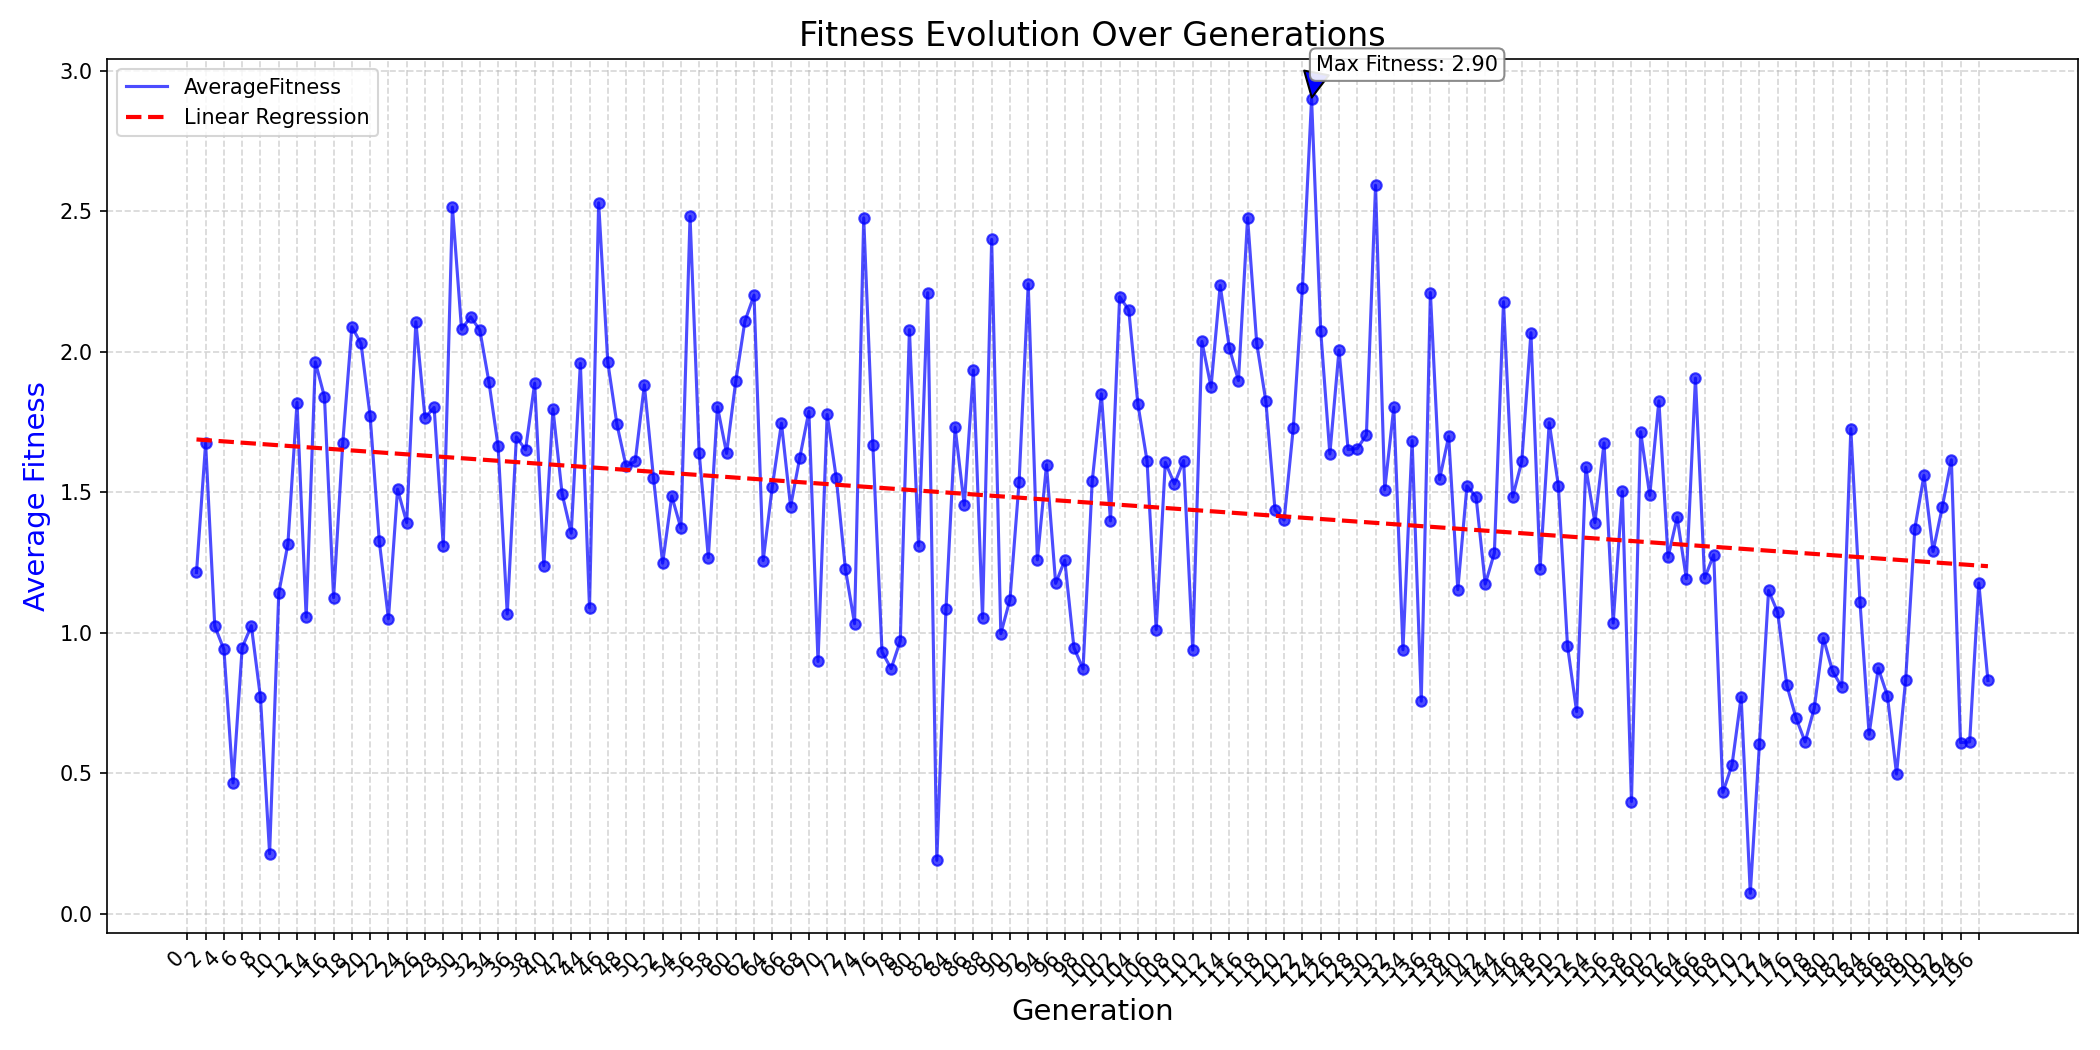
\includegraphics[width=0.4\textwidth]{figures/fitness_ann_adv_plot_4n.png}
    \caption{Average Fitness evolution over 300 generations for 4-neuron network}
    \label{fig:annadv}
\end{figure}

\begin{figure}[H]
    \centering
    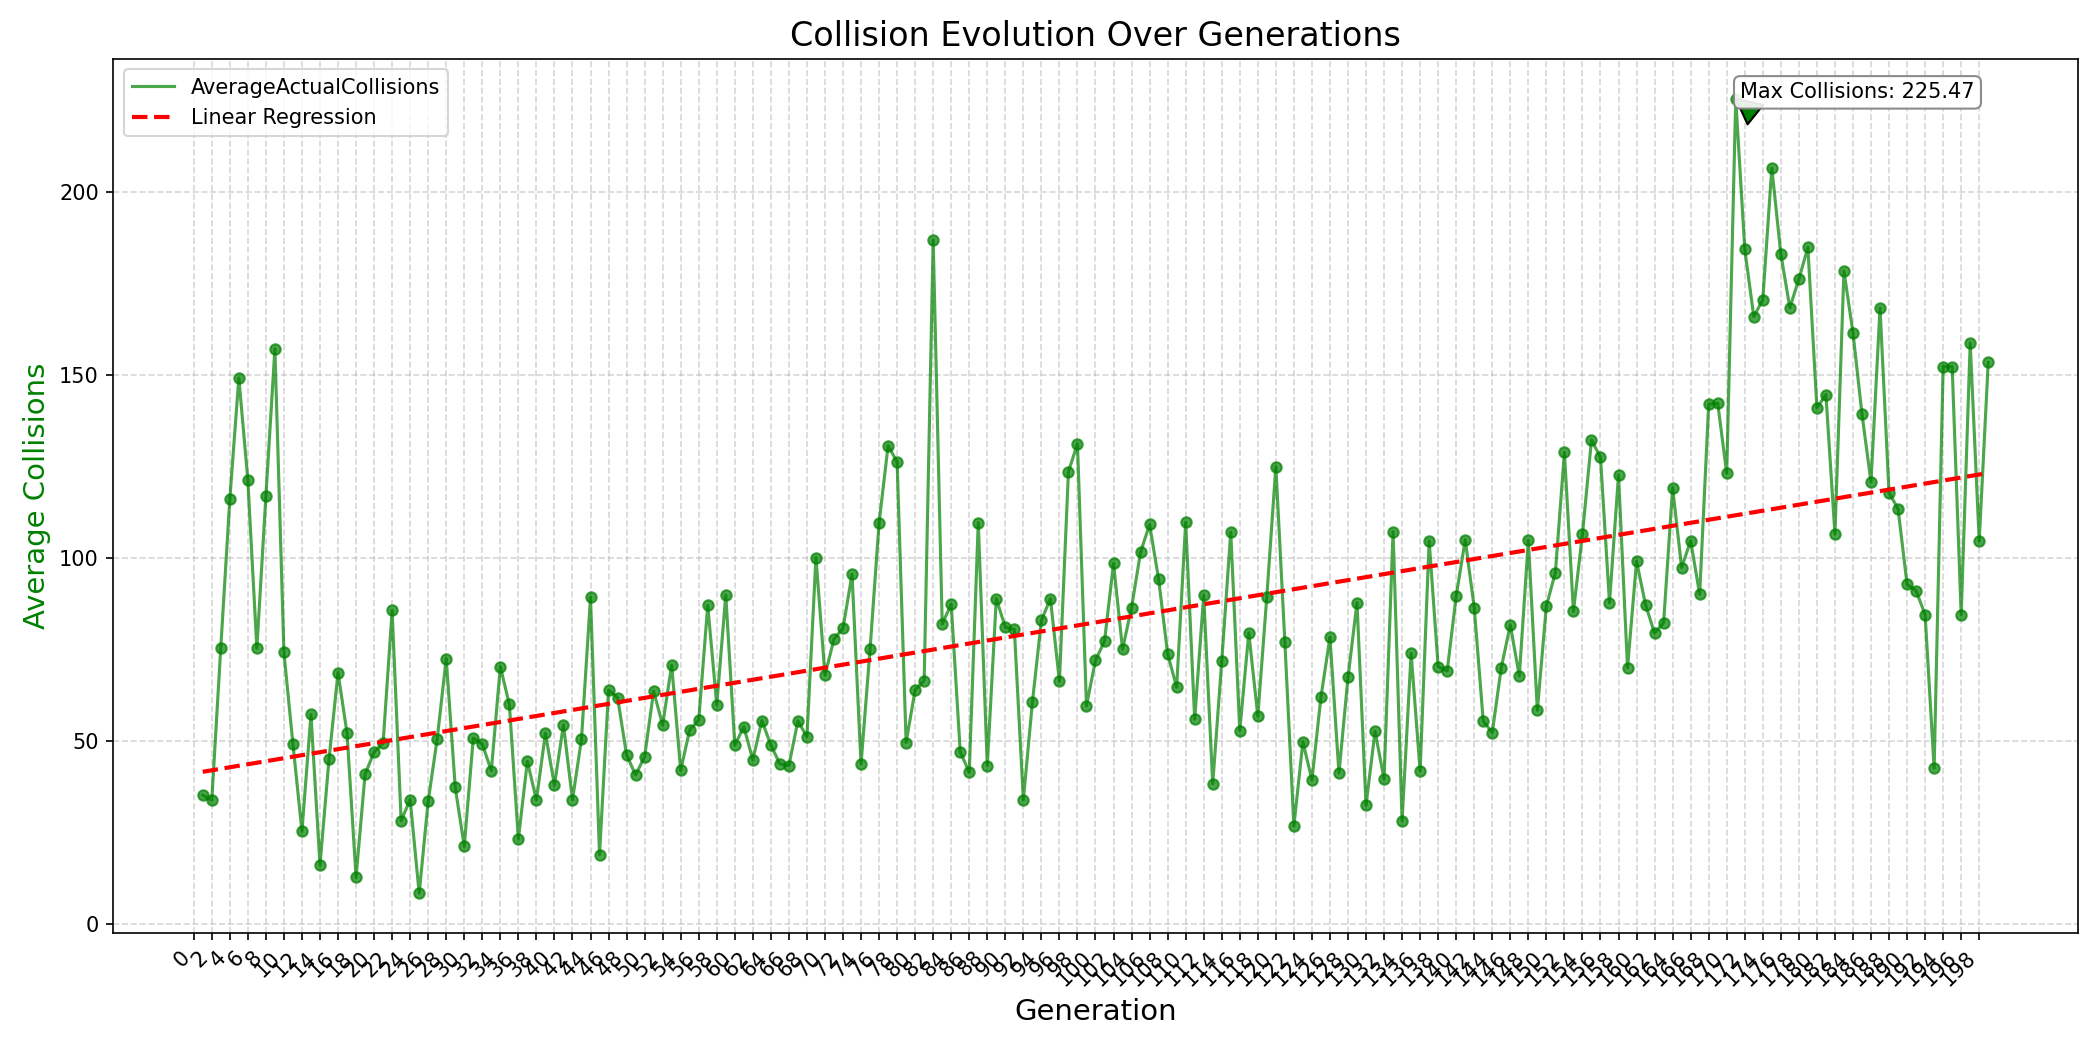
\includegraphics[width=0.4\textwidth]{figures/fitness_ann_adv_plot_4n_collisions.png}
    \caption{Collision count over 300 generations for 4-neuron network}
    \label{fig:annadv2}
\end{figure}

For the test with the 4 neurons it did not perform very well as we can see the figure \ref{fig:annadv} where the fitness dropped as the collisions got higher \ref{fig:annadv2}, we believe this happened because because it did not learn soon enough to avoid objects in the line, or avoid objects while traveling to the line, for the 10 neurons the test performed better as we can see in \ref{fig:annadv} where it had a inverse result, the collisions got lower as demonstrated in the figure \ref{fig:annadv4} and the fitness improved over time \ref{fig:annadv3}, confirming our expectation that the 10 neurons network would perform better in this conditions.

\begin{figure}[H]
    \centering
    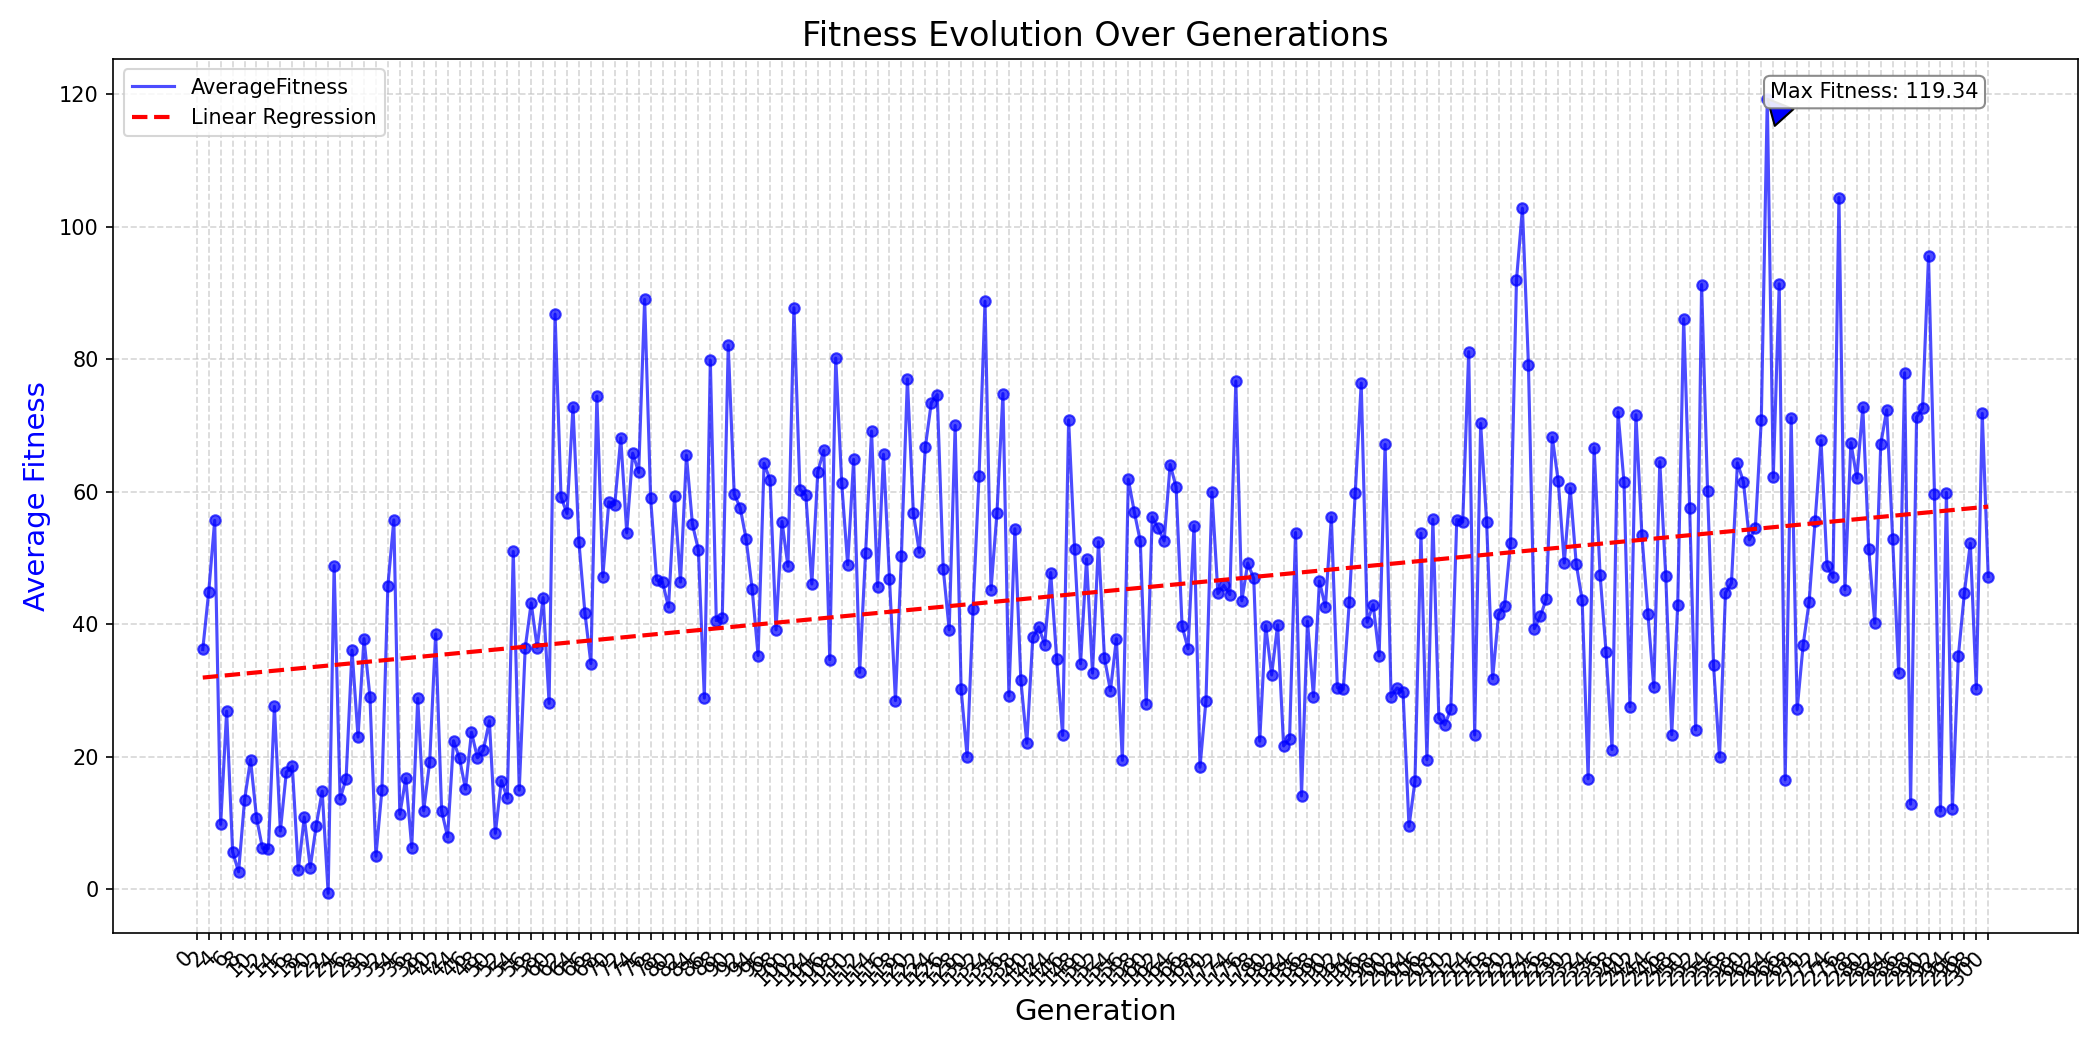
\includegraphics[width=0.4\textwidth]{figures/fitness_ann_adv_plot_10n.png}
    \caption{Average Fitness evolution over 300 generations for 10-neuron network}
    \label{fig:annadv3}
\end{figure}

\begin{figure}[H]
    \centering
    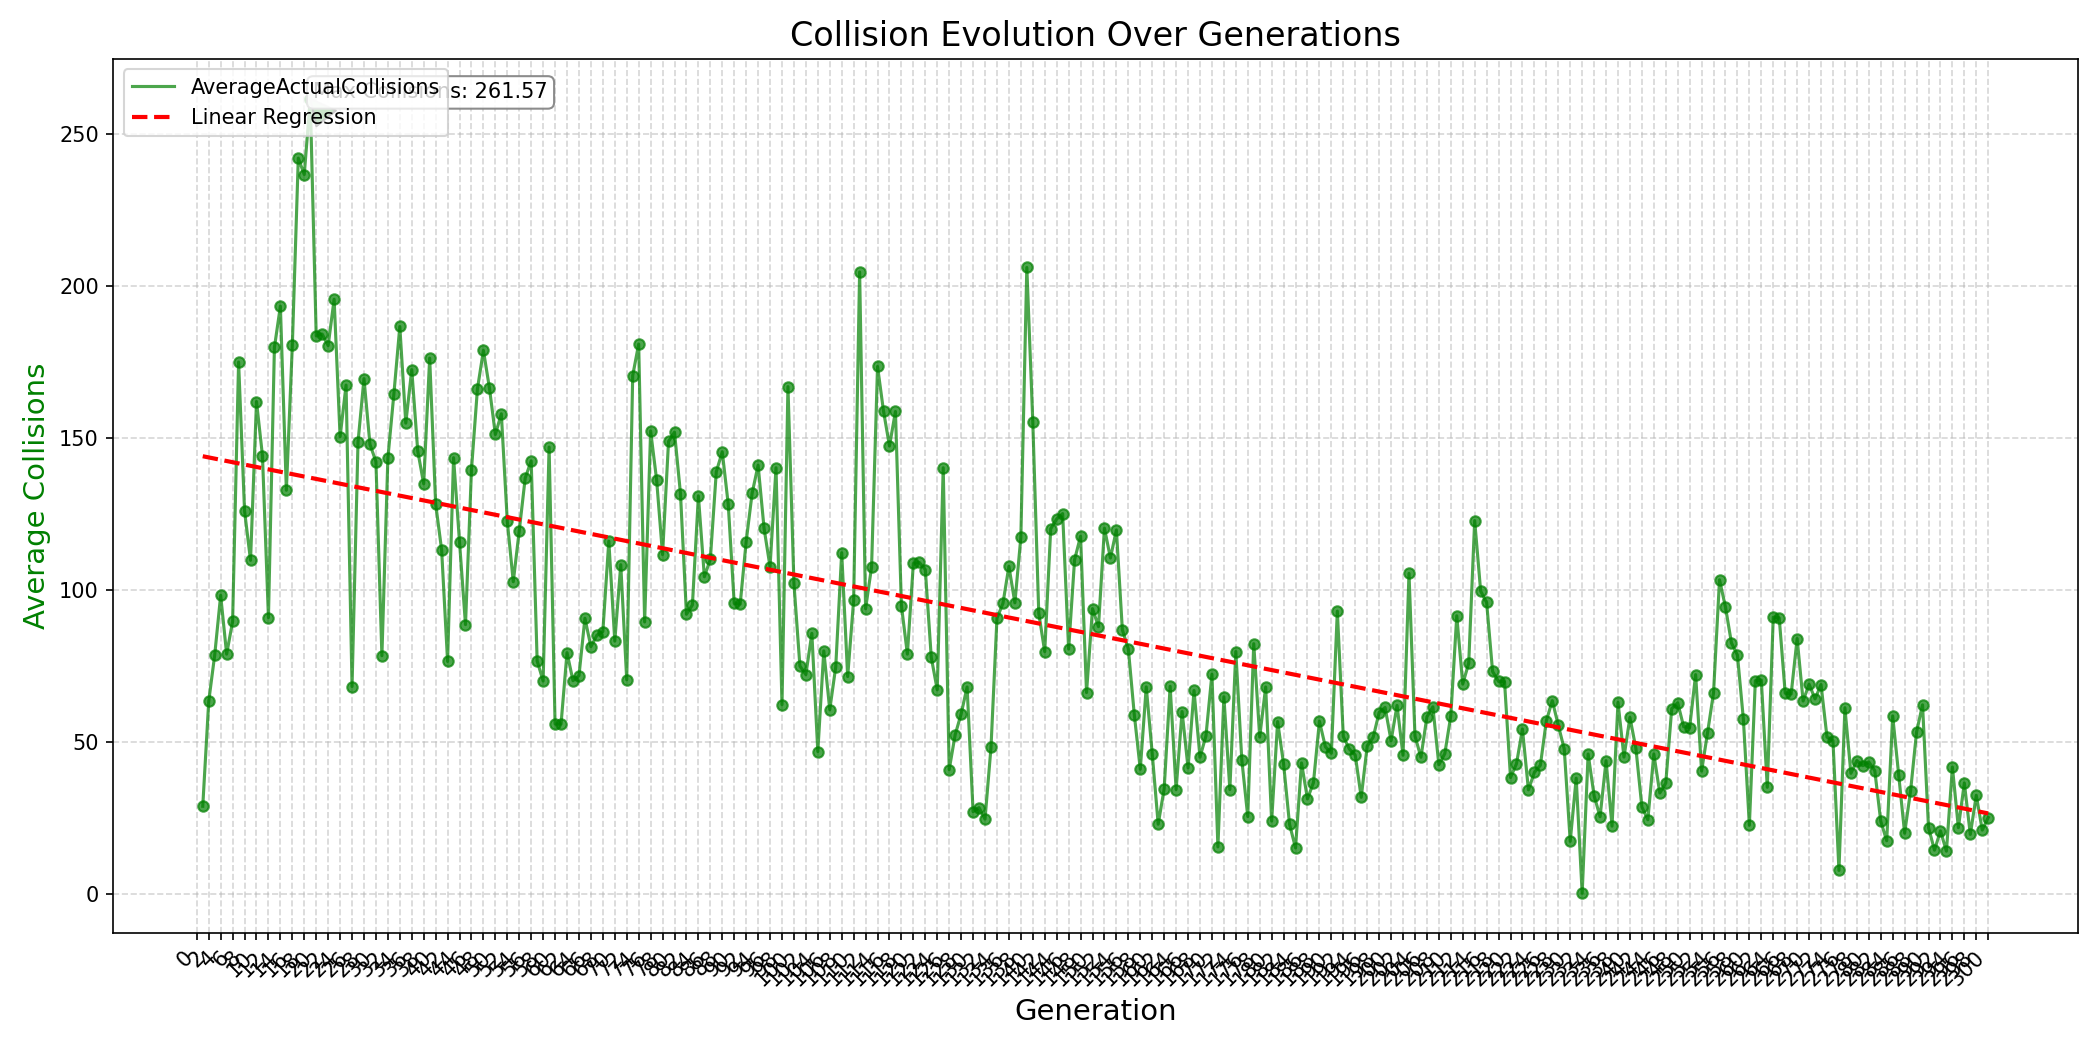
\includegraphics[width=0.4\textwidth]{figures/fitness_ann_adv_plot_10n_collisions.png}
    \caption{Collision count over 300 generations for 10-neuron network}
    \label{fig:annadv4}
\end{figure}

\subsection{Part B: PPO Implementation}

The performance of the Deep Reinforcement Learning agents was evaluated comparing the standard Proximal Policy Optimization (PPO) with its recurrent variant (RecurrentPPO). The analysis focused on the impact of the reward structure, activation functions (ReLU vs. Tanh), and environment randomization.

\subsubsection{PPO Performance with ReLU Activation}

The training results for PPO agents using the ReLU activation function are presented in Figure~\ref{fig:ppo_relu}. The configuration with penalties and randomized obstacles (\texttt{PPO\_ReLU\_randObs\_penalty}) achieved the highest average reward, outperforming all other variants. In contrast, configurations without penalties (\texttt{\_noPenalty}) learned suboptimal policies, often maximizing reward by remaining stationary, which highlights the necessity of a well-shaped reward function for meaningful learning.

\begin{figure}[H]
    \centering
    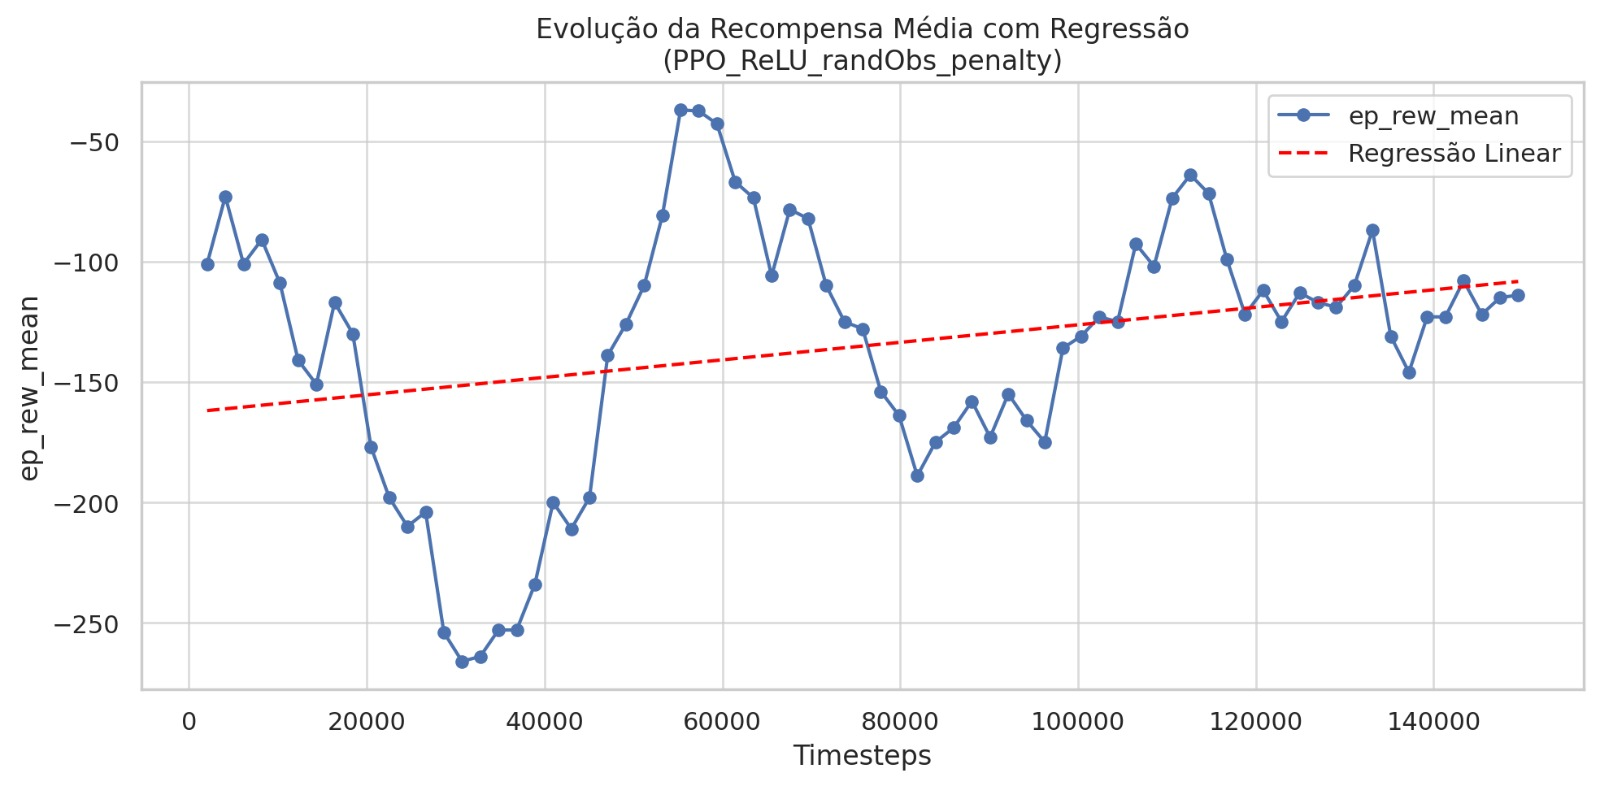
\includegraphics[width=0.4\textwidth]{figures/PPO_relu.jpeg}
    \caption{Fitness evolution over generations: evolutionary Braitenberg machine}
    \label{fig:ppo_relu}
\end{figure}
\subsubsection{PPO Performance with Tanh Activation and Comparative Insights}

Figure~\ref{fig:ppo_tanh} shows the performance of PPO agents using the Tanh activation function. While these agents achieved reasonable performance (\texttt{fixedObs}), their effectiveness degraded significantly when faced with randomized obstacles, meaning that the tanh function, in this context, was less capable of producing a generalizable policy.

This shows that the best-performing model for was the one combining PPO with ReLU, with a penalty system, and domain randomization.

\begin{figure}[H]
    \centering
    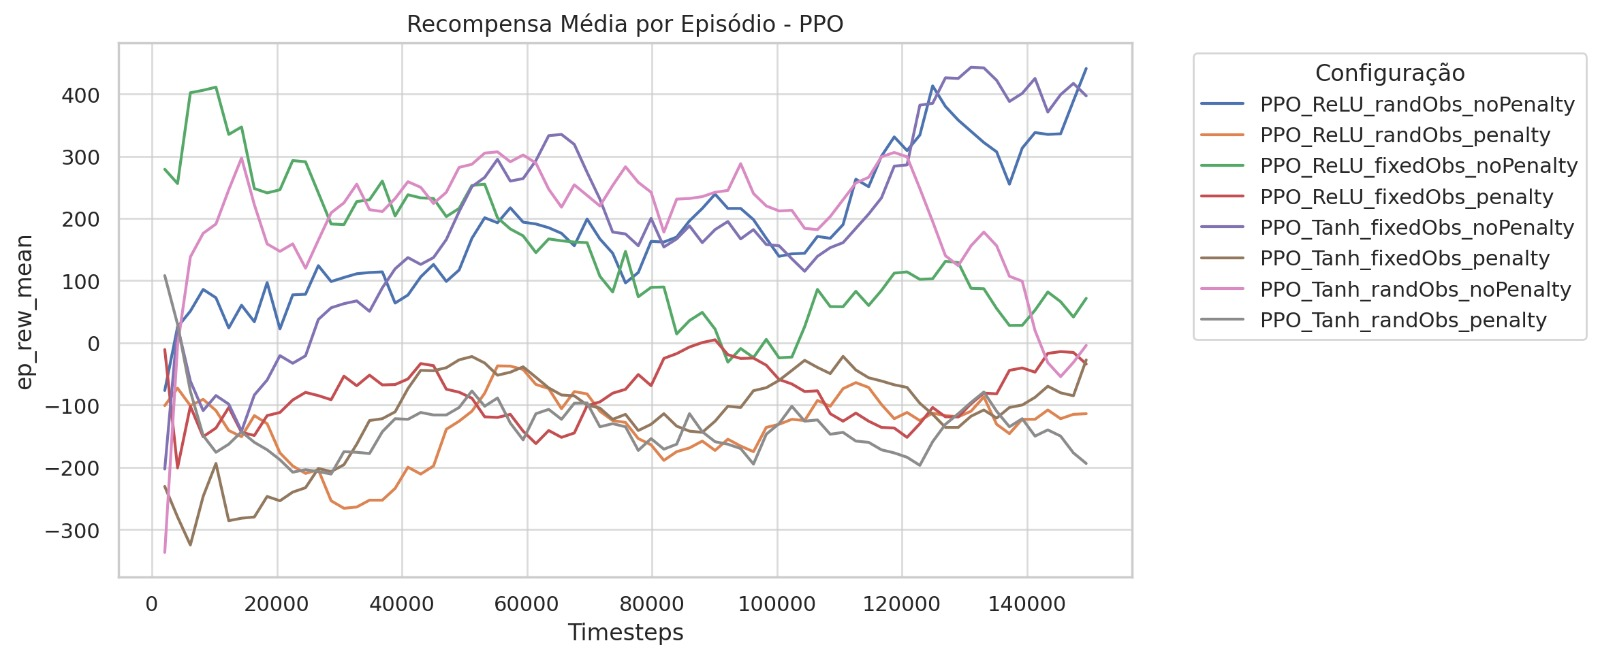
\includegraphics[width=0.45\textwidth]{figures/PPO_tanh.jpeg}
    \caption{Fitness evolution over generations: evolutionary Braitenberg machine}
    \label{fig:ppo_tanh}
\end{figure}

\subsubsection{Comparative Analysis with RecurrentPPO}

RecurrentPPO (RPPO) was also used, the obtained results can be seen in Figure~\ref{fig:rppo}, but the correspond to the contrary of the initial hypothesis.

\begin{figure}[H]
    \centering
    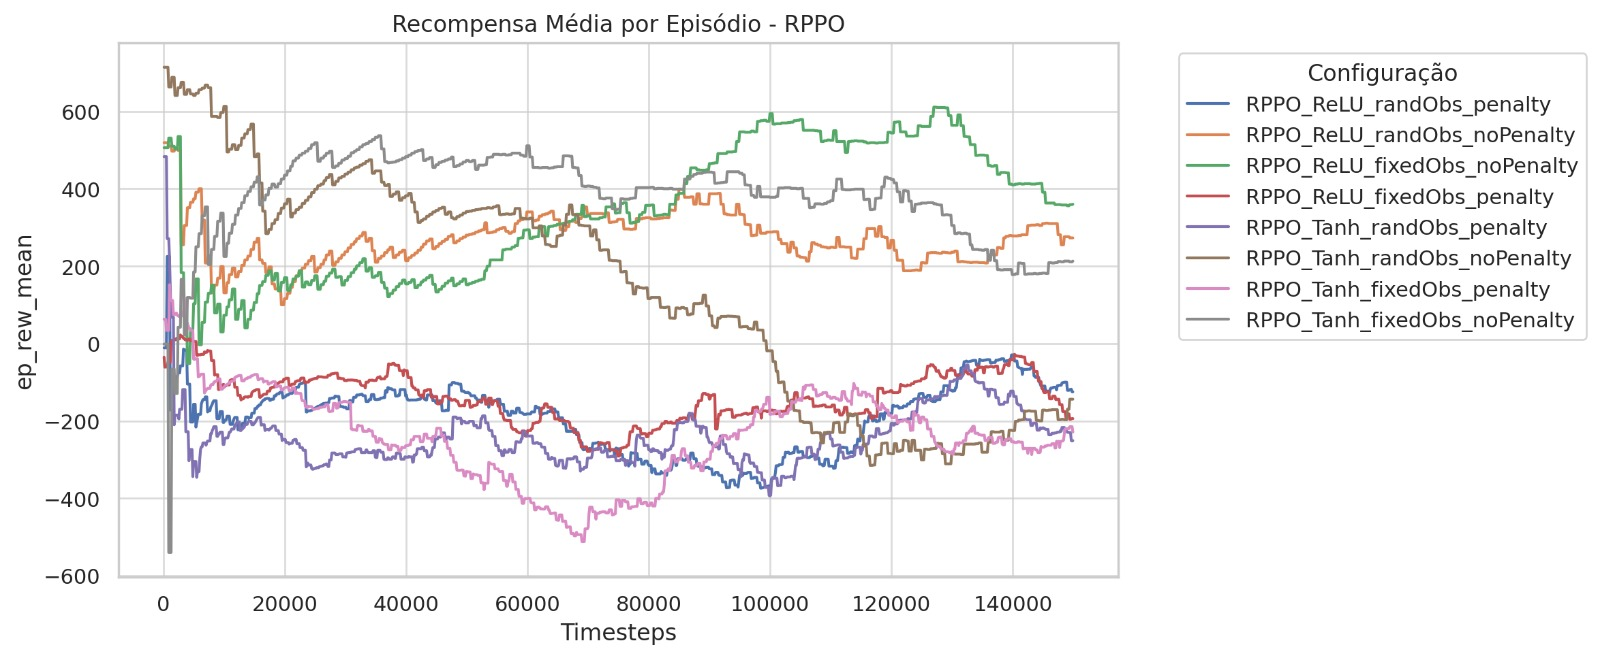
\includegraphics[width=0.45\textwidth]{figures/RPPO_Relu.jpeg}
    \caption{Fitness evolution over generations: evolutionary Braitenberg machine}
    \label{fig:rppo}
\end{figure}

The RPPO agents exhibited much greater training instability and failed to consistently outperform their simpler, non-recurrent counterparts. 

This outcome suggests that for this navigation task, the additional complexity of the recurrent network was not beneficial and may have even hindered sample efficiency. The purely reactive \texttt{MlpPolicy} of the standard PPO was sufficient to learn an effective policy from the sensory information.

% \subsection{Proximal Policy Optimization}

% \begin{figure}[H]
%     \centering
%     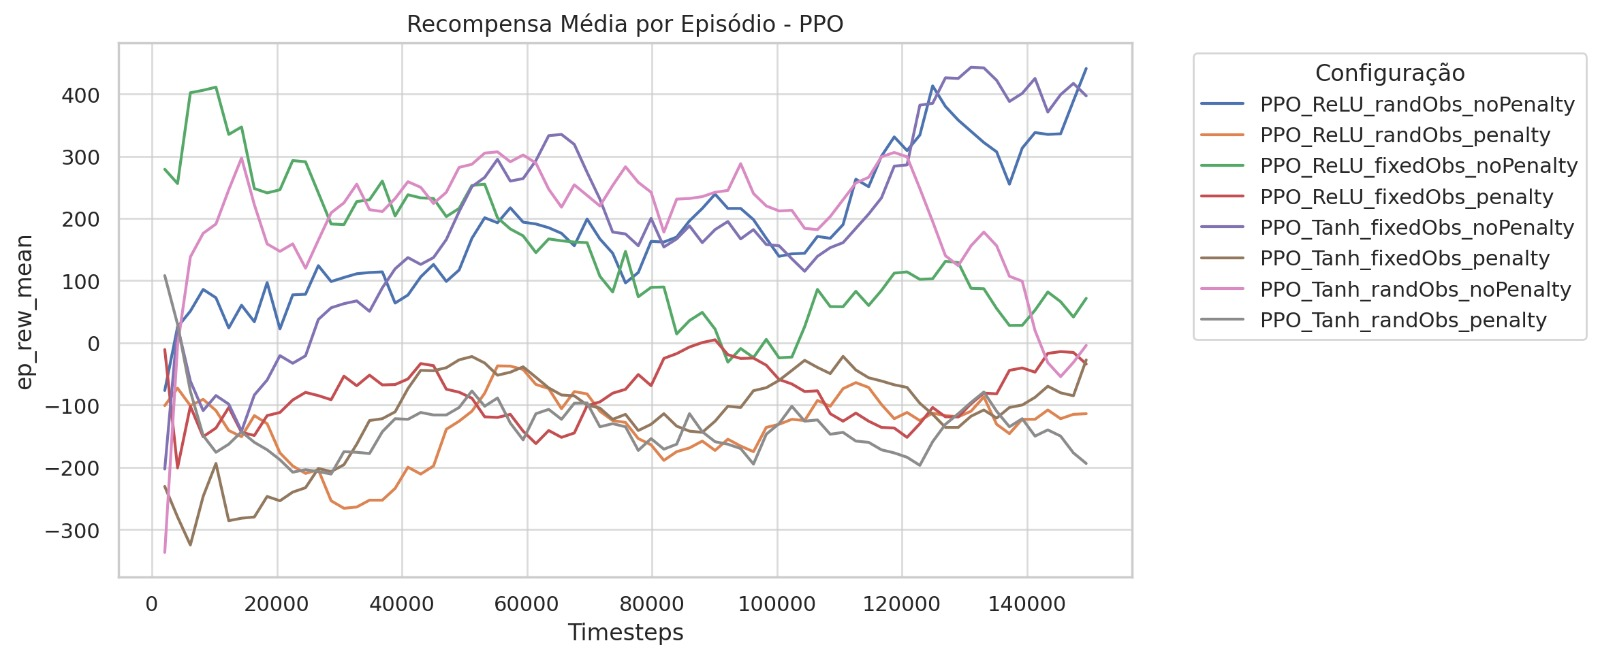
\includegraphics[width=0.4\textwidth]{figures/PPO_tanh.jpeg}
%     \caption{Fitness evolution over generations: evolutionary Braitenberg machine}
%     \label{fig:ppo_tanh}
% \end{figure}

% \begin{figure}[H]
%     \centering
%     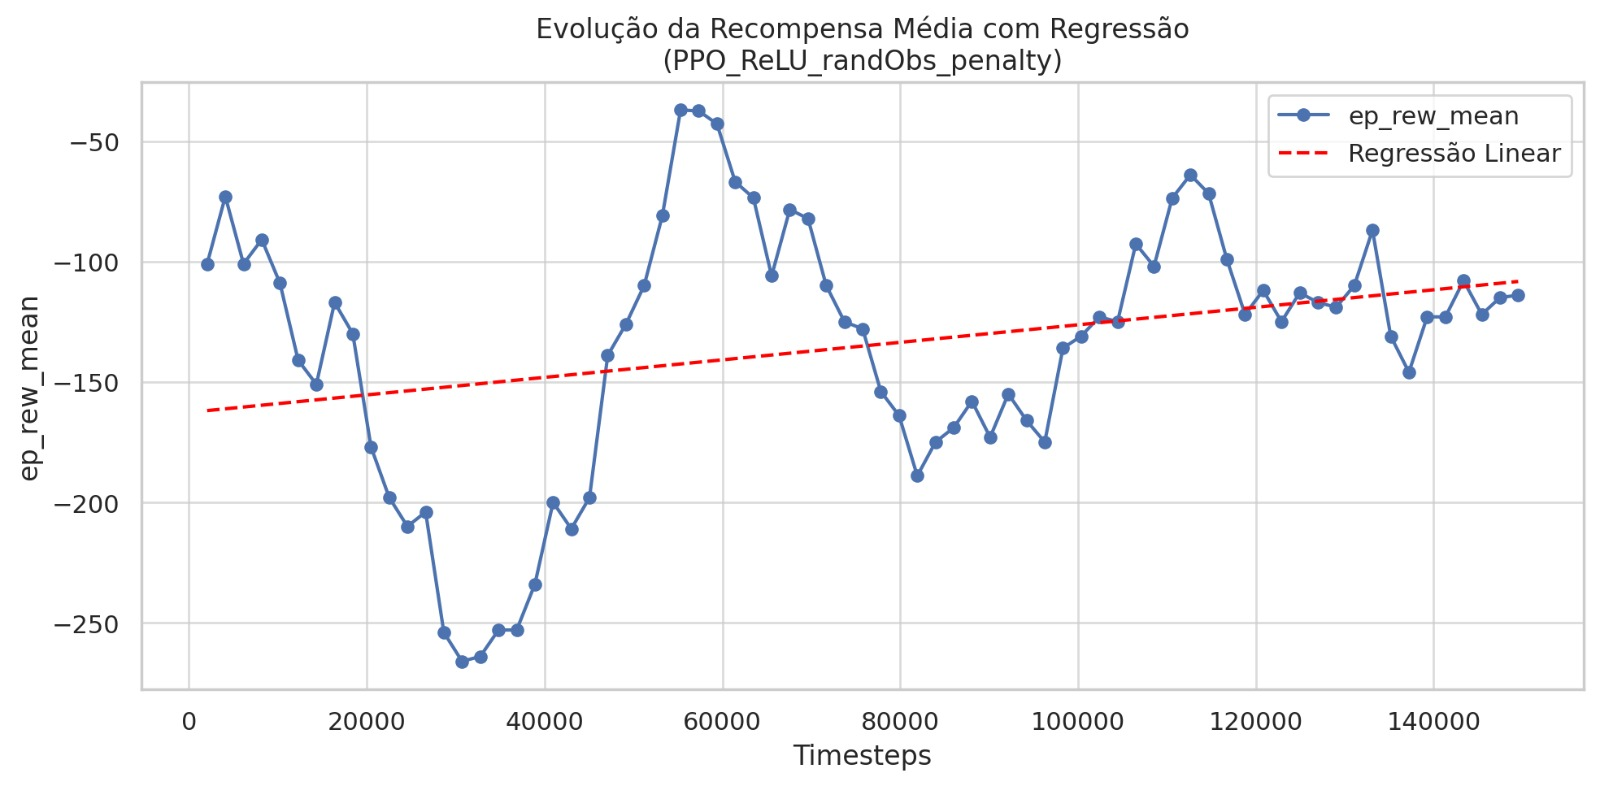
\includegraphics[width=0.4\textwidth]{figures/PPO_relu.jpeg}
%     \caption{Fitness evolution over generations: evolutionary Braitenberg machine}
%     \label{fig:ppo_relu}
% \end{figure}


% \subsection{Recurrent Proximal Policy Optimization}
% \begin{figure}[H]
%     \centering
%     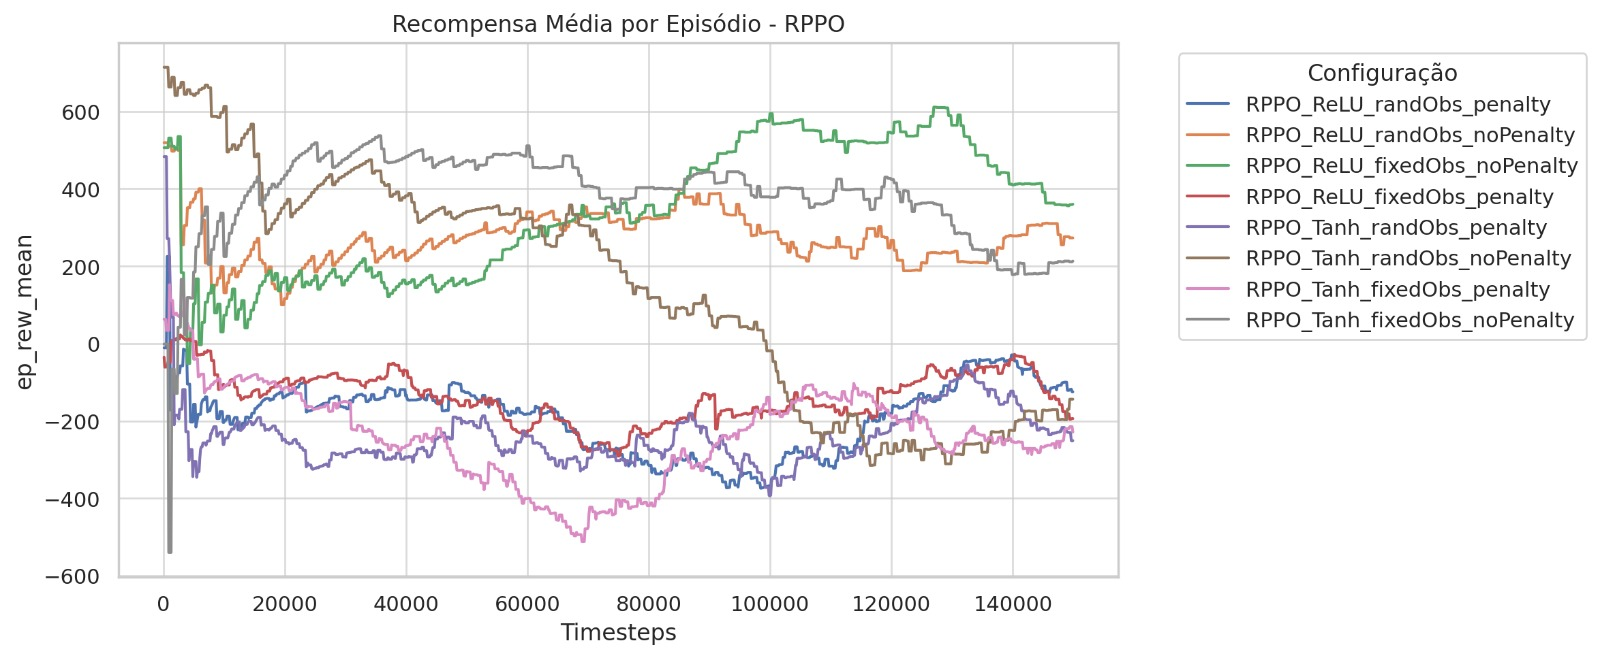
\includegraphics[width=0.4\textwidth]{figures/RPPO_Relu.jpeg}
%     \caption{Fitness evolution over generations: evolutionary Braitenberg machine}
%     \label{fig:rppo}
% \end{figure}

\section{Conclusion}

This project demonstrated that while both classical and modern approaches can yield effective controllers for Thymio robots, their performance depends on task complexity and algorithm suitability. Evolutionary algorithms and simple ANNs performed well in structured environments, but struggled with generalization. Deep Reinforcement Learning, particularly PPO with ReLU and well-shaped rewards, achieved robust performance in randomized settings. However, adding memory through Recurrent PPO introduced instability, showing that more complex models are not always advantageous for relatively simple navigation tasks.

\bibliographystyle{elsarticle-harv}
\bibliography{main}

\appendix
\section{Additional Graphs}
\label{sec:appendix}

\begin{figure}[H]
    \centering
    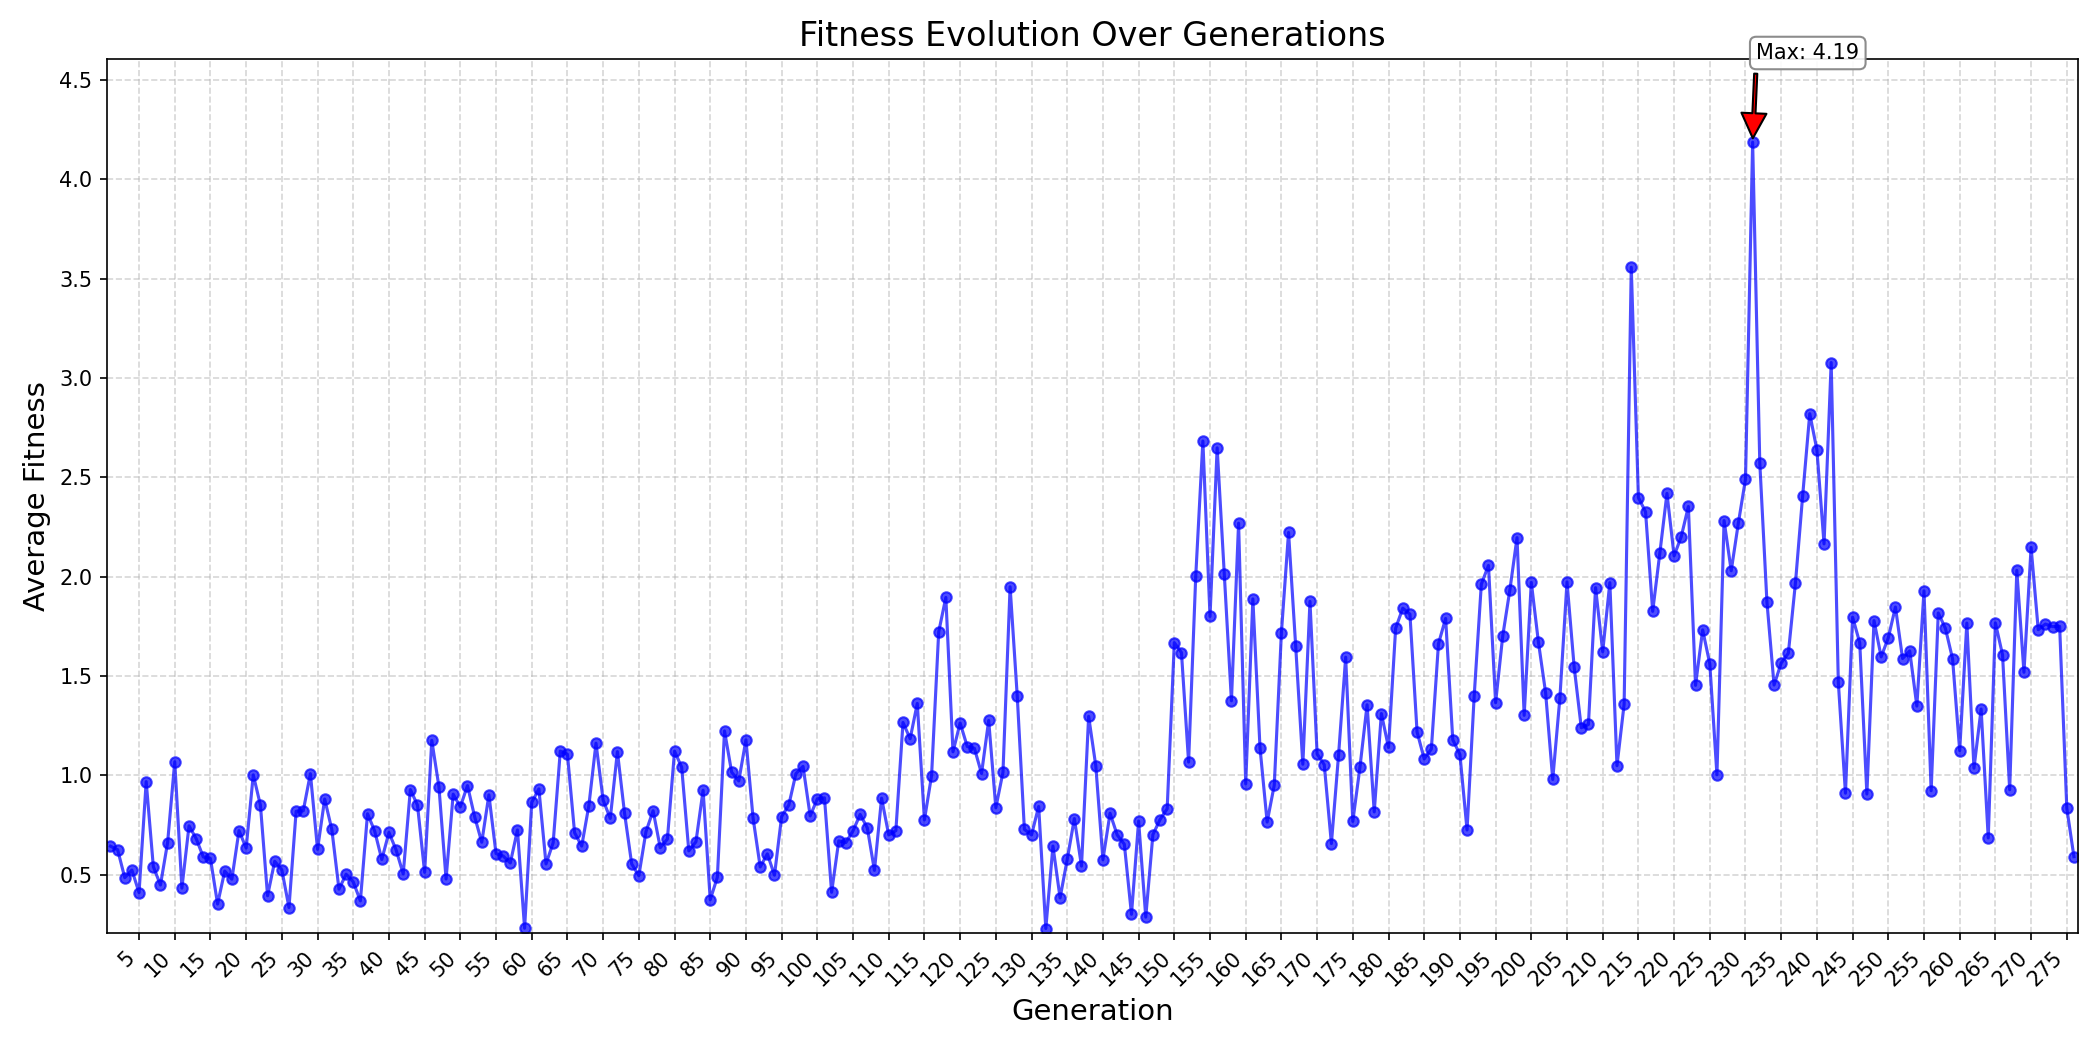
\includegraphics[width=1\linewidth]{figures/ann_simples_3runs_params2.png}
    \caption{Simple ANN, where fitness of each individual was calculated as an average of 3 runs of that individual.}
    \label{fig:ann_simples_3runs_params2}
\end{figure}

\begin{figure}[H]
    \centering
    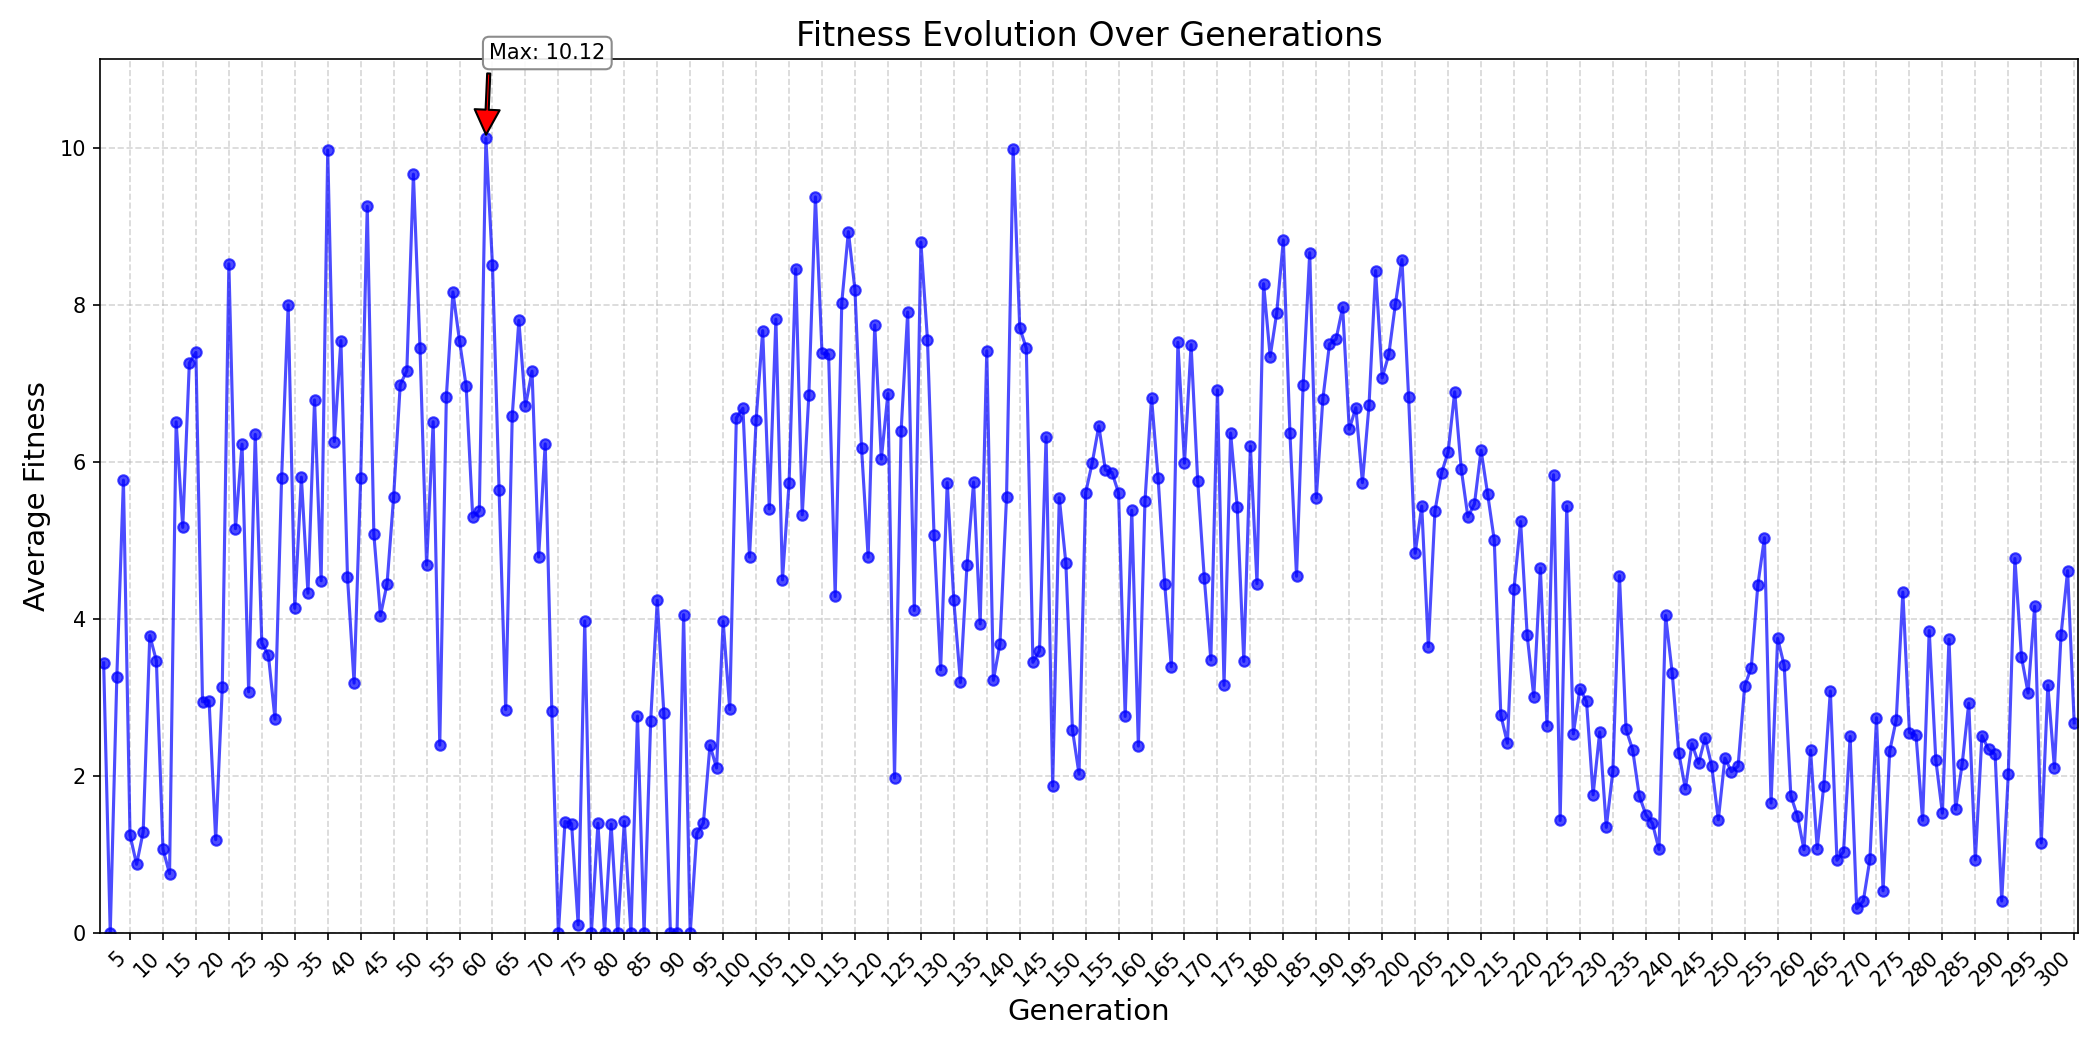
\includegraphics[width=1\linewidth]{figures/ann_simples_leonor_params2.png}
    \caption{Simple ANN with adaptive fitness to encourage exploration in the beginning and exploitation in the end.}
    \label{fig:enter-label}
\end{figure}

\begin{figure}[H]
    \centering
    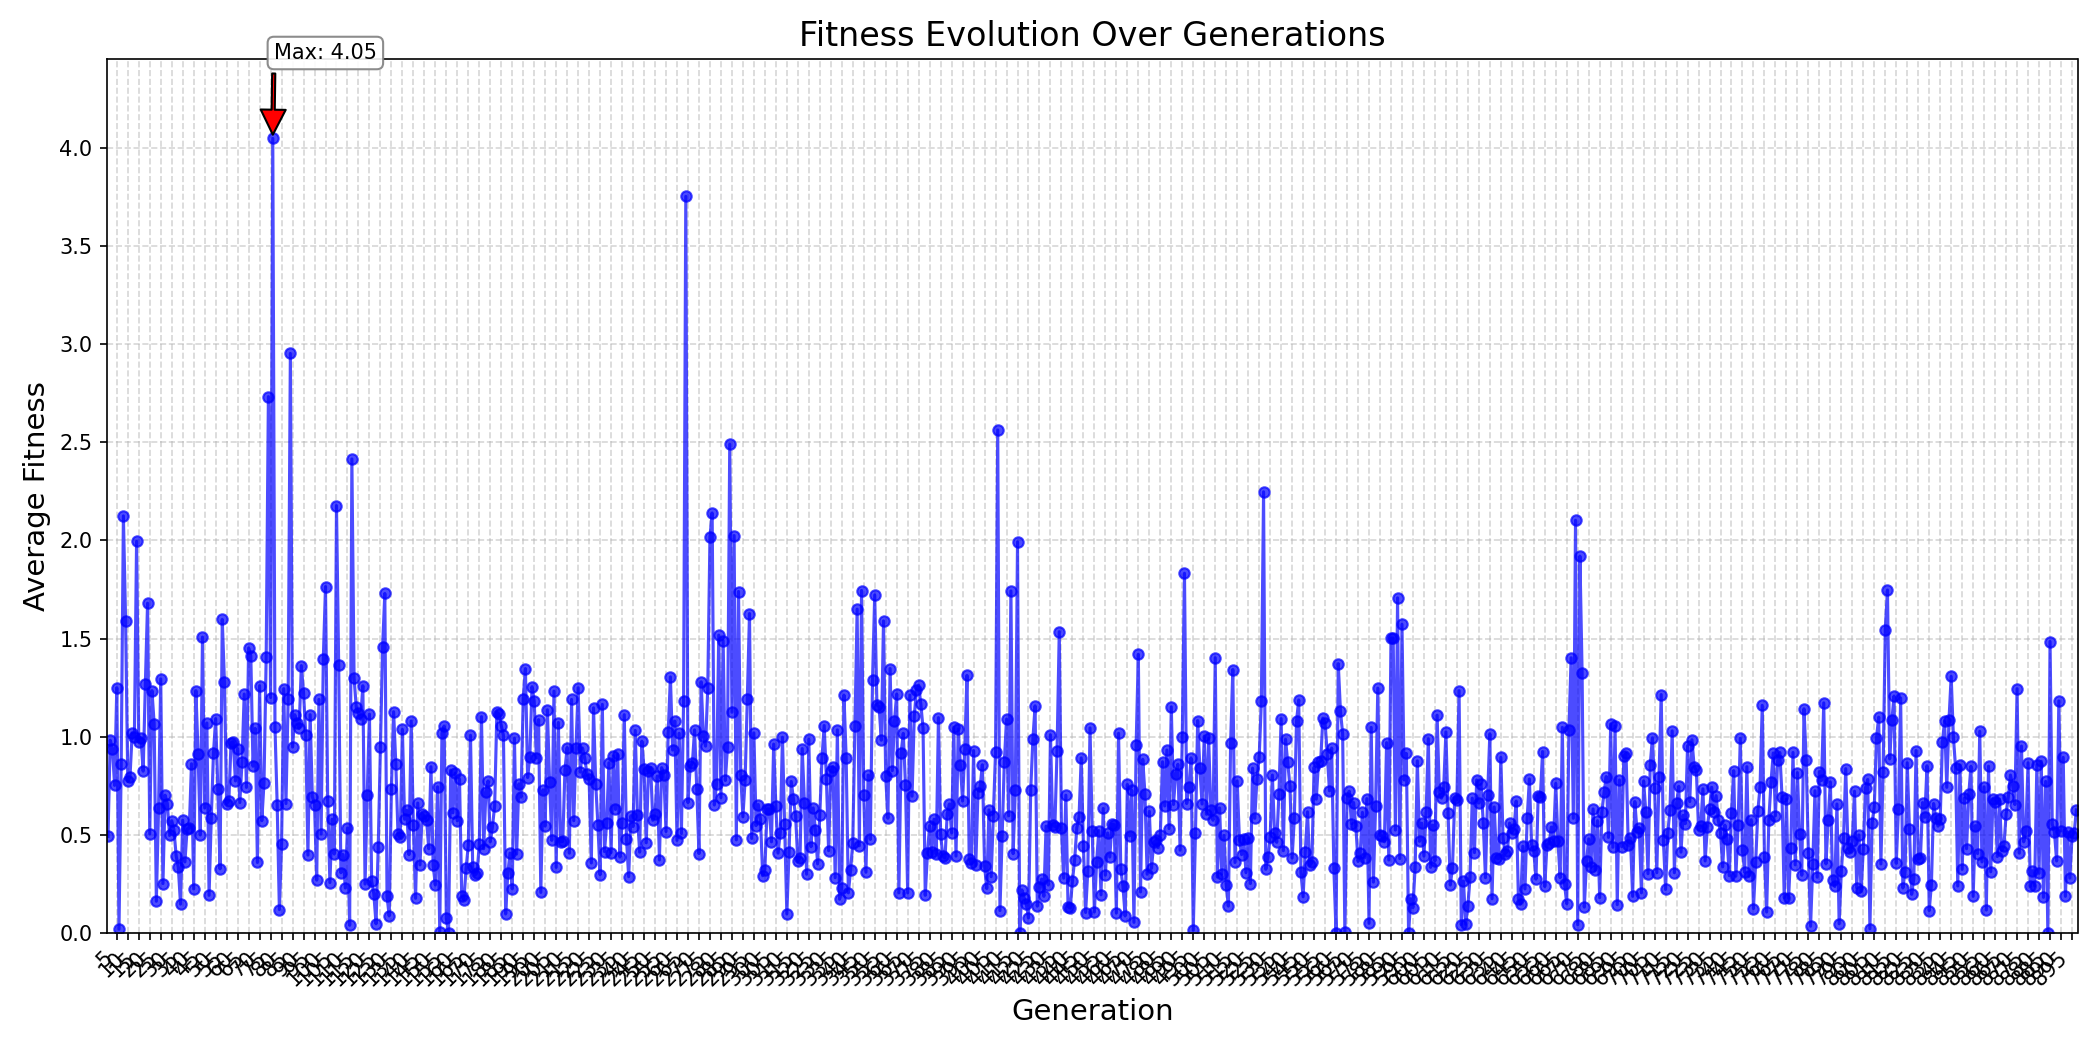
\includegraphics[width=1\linewidth]{figures/aold_ann_simples_params2.png}
    \caption{Earlier simple ANN iteration}
    \label{fig:enter-label}
\end{figure}

\begin{figure}[H]
    \centering
    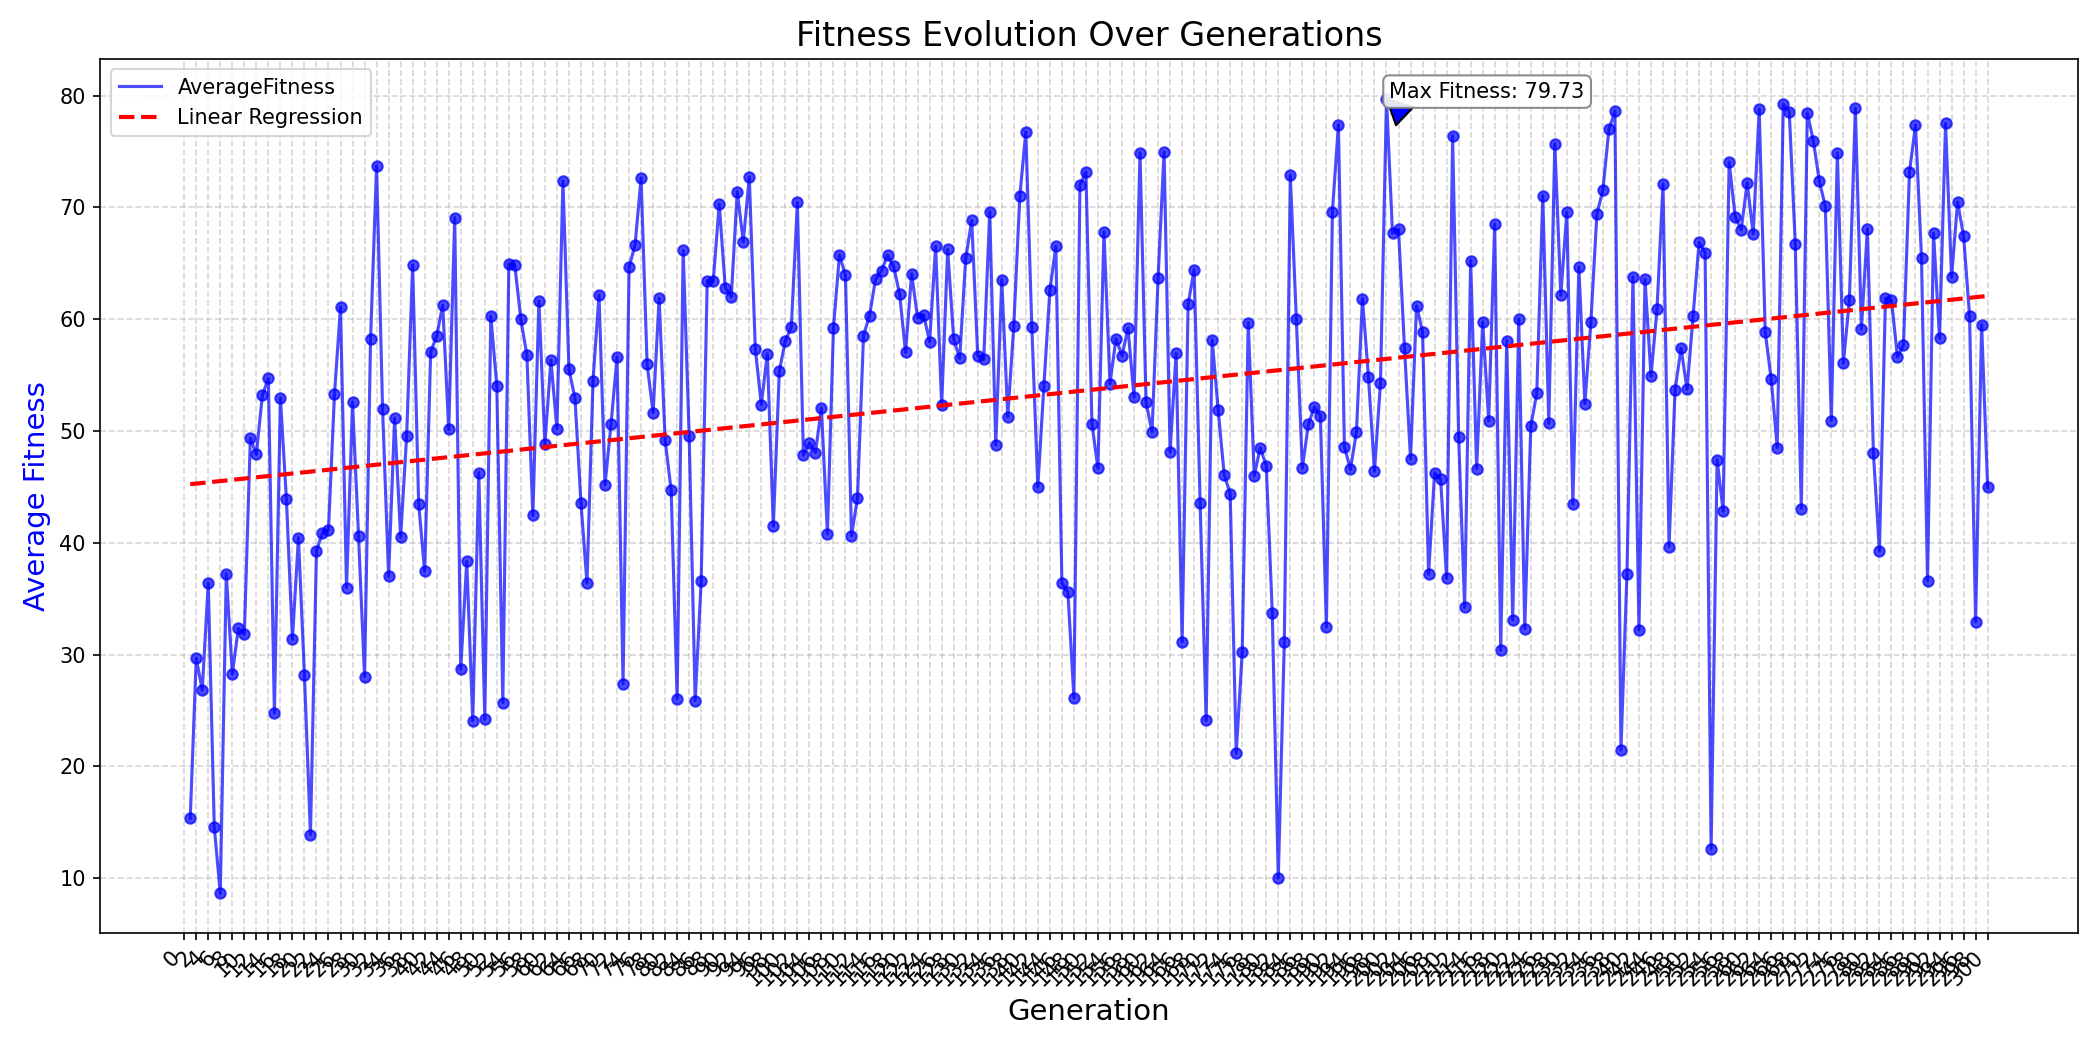
\includegraphics[width=1\linewidth]{figures/APPENDIX_ann_advance_best_first.png}
    \caption{Earlier advanced ANN iteration, before calculation of distance between steps}
    \label{fig:enter-label}
\end{figure}

% Example content:
% \begin{figure}[h]
%     \centering
%     \includegraphics[width=0.7\textwidth]{figures/example-graph}
%     \caption{Example graph for parameter tuning.}
%     \label{fig:example-appendix}
% \end{figure}

\end{document}

